Les activités de recherches présentées dans la section \ref{sec:doctorat} ont été menées au GeM\footnoteref{GeM} sur le site de l'{\'E}cole Centrale de Nantes.
Elles s'inscrivaient dans le cadre de ma thèse de doctorat (bourse MESRI) dirigée par Laurent Stainier\footnoteref{GeM} et Thomas Heuzé\footnote{\label{GeM}Institut de recherche en Génie Civil et Mécanique}.

L'activité \ref{sec:post-doc} relève quant à elle de mes travaux de postdoc au MSSMat à CentraleSupélec, financés par le Labex LaSIPS\footnote{https://www.universite-paris-saclay.fr/en/recherche/laboratoires-et-equipements/laboratoires-dexcellence/labex-lasips}, en collaboration avec Bing Tie\footnote{\label{MSSMat}Laboratoire de Mécanique des Sols, Structures et Matériaux}, Anne-Sophie Mouronval\footnoteref{MSSMat}, Jean-Hubert Schmitt\footnoteref{MSSMat}, Denis Aubry\footnoteref{MSSMat} et Denis Solas\footnote{Institut de Chimie Moléculaire et des Matériaux d'Orsay (ICMMO, Université Paris-Saclay)}  dans le projet ModUS3D\footnote{Modélisation des ondes UltraSonores en 3D}.

Enfin, la section \ref{sec:post-doc_CEA} est consacrée aux activitées que je mène actuellement au CEA/LC2M\footnoteref{LC2M} dans le cadre d'un second postdoc encadré par Laurent Dupuy\footnote{\label{LC2M}Laboratoire d'étude du Comportement Mécanique des Matériaux} et Lionel Gélébart\footnoteref{LC2M}.
Ces travaux s'inscrivent dans le projet H2020 M4F\footnote{Multiscale modeling for fusion and fission materials: http://www.h2020-m4f.eu/} et se font en forte interaction avec Marc Fivel\footnote{\label{SIMap}Laboratoire de Science et Ingénierie des Matériaux et Procédés -- Grenoble INP} de l'université de Grenoble, et  Prita Pant\footnote{\label{ITT}Department of Metallurgical Endineering and Materials Science} et M.P. Gururajan\footnoteref{ITT} de l'\textit{Indian Institute of Technology of Bombay}.


% \begin{refsection}[Biblio.bib]
%   \subsection{Simulation Eulérienne du procédé FSW}
% % Simulation eulérienne de l'extrusion de couches de matière au cours du procédé FSW due à un défaut d'excentrement de l'outil
%   \label{sec:pre-doc}
%   \paragraph{Motivations : }
$\newline$
Le procédé de soudage par friction et malaxage (\textit{Friction Stir Welding - FSW}) est devenu populaire grâce à sa capacité à assembler à l'état solide, et sans apport de matière, des matériaux réputés difficilement soudables.
Plus spécifiquement, je me suis concentré sur la configuration ``bout-à-bout'' dans laquelle deux plaques sont placées de façon jointive sur une de leur tranche.
Un outil en rotation rapide autour de l'axe perpendiculaire aux plaques (de 500 à 2000 tr/min) se déplace alors le long de l'interface, transformant ainsi la matière en pâte malléable par échauffement (températures de l'ordre de 500$^{o}$C) et opérant le mélange des deux pièces initialement disjointes.
Des études expérimentales du procédé \cite{Krish} ont permis de mettre en évidence la formation de structures en ``oignons'' dans la zone fortement malaxée, c'est-à-dire d’ellipses concentriques observées au niveau du joint soudé dans une coupe transversale.
La formation des \textit{onion rings} a ensuite été attribuée à un défaut d’excentrement de l’outil lors du soudage \cite{Grat}.
L'objectif de mes travaux était de mettre en évidence le phénomène de formation des \textit{onion rings} numériquement en proposant une simulation tridimensionnelle du FSW.

\paragraph{Contributions : }
$\newline$
\begin{figure}[h!]
  \centering
  \begin{tikzpicture}[scale=1]
  \begin{groupplot}[group style={group size=2 by 1,% columns by rows
      ylabels at=edge left, yticklabels at=edge left,
      horizontal sep=2.ex,
      vertical sep=2ex,},
    enlargelimits=0,
    xmin=0.,xmax=1., ymin=-0.,ymax=1.
    ,axis on top,scale only axis,width=0.45\linewidth
    ,xtick=\empty,ytick=\empty,
    colorbar style={
      title style={
        font=\footnotesize,
        at={(1,.5)},
        anchor=north west
      },yticklabel style={font=\footnotesize}
      ,at={(current axis.south east)},anchor=south west
    },colormap name=tol
    ]
    %% FIRST ROW (time 1 = 5.10e-4s)
    %%% RANGE -8.6e9 -- 0.57e9
    % \nextgroupplot[title={Température}]\addplot graphics[xmin=0.,xmax=1., ymin=-0.,ymax=1.] {pngFigures/Stationnaire.png};
    \nextgroupplot[title={Température}]\addplot graphics[xmin=0.,xmax=1., ymin=-0.,ymax=1.] {pngFigures/Stationnaire_croped.png};
    \nextgroupplot[title={Lignes de courant}]\addplot graphics[xmin=0.,xmax=1., ymin=-0.,ymax=1.] {pngFigures/Streamline_classical.png};
    
  \end{groupplot}
\end{tikzpicture}



%%% Local Variables:
%%% mode: latex
%%% TeX-master: "../manuscript"
%%% End:

  \caption{Résultats de simulations numériques tridimensionelles du procédé de soudage par friction/malaxage avec un défaut d'excentrement de l'outil rotatif.}
  \label{fig:FSW}
\end{figure}
Afin d'éviter les étapes coûteuses de re-maillage ou de re-zonage impliquées par les forts taux de déformations en jeu pour des approches Lagrangienne ou \textit{Arbitrary-Lagrange-Euler} (ALE) \cite{Bas,Guerdoux,Heuz,Feul2,Fourment}, j'ai proposé une formulation purement Eulérienne du problème.
L'originalité de la modélisation consiste en la représentation de la géométrie de l'outil au moyen de fonctions de niveau, combinée à l'utilisation de la technologie X-FEM \cite{Moes99}.
La cinématique de l'outil comprenant le défaut d'excentrement est imposée le long de l'interface outil/matière.
La matière est modélisée par un fluide très visqueux dont les propriétés mécaniques dépendent de la température, elle-même influencée par la dissipation plastique et le frottement au bord de l'outil.
%On considère donc un problème thermo-mécanique couplé fortement, résolu de manière étagée dans une librairie développée au GeM et qui prend en compte le formalisme X-FEM.
La résolution numérique du problème thermo-mécanique couplé fortement était effectuée grâce à deux codes de calcul développés au GeM, l'un gérant l'intégration des lois constitutives par solveurs variationnels, et l'autre prenant en compte le formalisme X-FEM. 
Le couplage entre les deux librairies était la première étape de mon travail.

Les premières simulations basées sur ce modèle ont conduit à des résultats satisfaisants (voir figure \ref{fig:FSW}).
L'échauffement dans la zone proche de l'outil est notable et les lignes de courant tracées rendent bien compte de l'entraînement de la matière.
Toutefois, la mise en évidence des \textit{onion rings} nécessite des travaux supplémentaires portant sur la reconstruction des trajectoires des points matériels et un choix de paramètres matériau favorable.


% Problèmes : jeu de paramètres pour le matériau, comportement fluide (Norton-Hoff), reconstruction des trajectoires lourdes avec paraview, prise en compte de la métallurgie?

%Fluide très visqueux (loi de Norton-Hoff) incompressible avec contact normal bilatéral entre l'outil et la matière avec glissement frottant;







%%% Local Variables:
%%% mode: latex
%%% TeX-master: "main"
%%% End:

%   \printbibliography[heading=subbibliography]
% \end{refsection}


\begin{refsection}
  \subsection{Propagation des ondes dans les solides hyperélastoplastiques}
  \label{sec:doctorat}
  Les travaux présentés dans ce qui suit prennent leur source dans les procédés de mise en forme de matériaux métalliques à haute vitesse.
{\`A} l'instar des problèmes d'impact, ces applications impliquent des ondes propageant des grandes déformations qui sont éventuellement irréversibles.
L'étude numérique de cette classe de problèmes, modélisés mathématiquement par des équations aux dérivées partielles hyperboliques, nécessite donc l'emploi de méthodes robustes pouvant gérer les grandes transformations et les ondes sans oscillations numériques dans les solutions.
Ce type d'études peut être mené afin de mieux comprendre la réponse des solides impliqués et d'optimiser les procédés de mise en forme.
Cette problématique a été déclinée en deux axes qui sont développés dans la suite.

\subsubsection{Extension de la Méthode des Points Matériels à l'approximation de Galerkin Discontinue}

\paragraph{Motivations:}
$\newline$
La résolution numérique des problèmes aux valeurs initiales et limites, auxquels les systèmes hyperboliques appartiennent, a été et est toujours principalement menée avec la Méthode des {\'E}léments Finis (FEM) \cite{Belytschko}.
Néanmoins, les grandes transformations impliquées conduisent à certaines limitations de la méthode:
\begin{itemize}
\item perte de précision pour les maillages très déformés si une approche Lagrangienne est utilisée,
\item nécessité d'utiliser des techniques de suivi d'interface et des étapes de projections diffusives des variables internes pour les approches Eulérienne ou ALE.
\end{itemize}

La Méthode des Points Matériels (MPM) \cite{Sulsky94}, en proposant une discrétisation du milieu solide basée sur des particules pouvant se déplacer dans une grille de calcul arbitraire, permet de s'affranchir des difficultés liées aux distorsions de maillage.
% Cependant, des étapes de projection des champs entre les particules et les n\oe uds du maillage conduisent soit à des oscillations parasites, soit à de la diffusion numérique \cite{Mass_Flip}.
Cependant, des oscillations parasites ou de la diffusion numérique peuvent apparaître selon la manière dont les champs sont projetés des n\oe uds du maillage vers les particules \cite{Mass_Flip}.

Par ailleurs, les intégrateurs temporels explicites couramment utilisés avec la FEM introduisent du bruit de haute fréquence dans le voisinage des fortes variations de champs, comme celles impliquées par des ondes.
L'introduction de l'approximation de Galerkin Discontinue (DG) \cite{NeutronDG} dans la FEM permet de supprimer ces oscillations en prenant en compte la structure mathématique des solutions des problèmes hyperboliques \cite{Cockburn}.
Toutefois, la DGFEM est également sujette aux problèmes liés aux grandes transformations.



L'objectif poursuivi dans cette partie est donc le développement d'une méthode numérique capable de suivre précisément les ondes dans les solides se déformant beaucoup.

\paragraph{Contributions:}
$\newline$ % formulation de la méthode
De manière analogue à la MPM, la DGMPM (\textit{Discontinuous Galerkin Material Point Method}) \cite{DGMPM} est basée sur la discrétisation d'un domaine solide en une collection de particules pouvant se déplacer dans une grille de calcul (voir figure \ref{fig:continuum}).
\begin{figure}[ht]
  \centering
  \begin{tikzpicture}[scale=0.25]
  % \draw[step=1.0,black,thin] (-3.,-1.) grid (3,4.);
  % \draw (-3,-1) -- (3,-1) -- (3,4) -- (-3,4) -- (-3,-1);
  \begin{scope}[scale=0.5]
    \draw (-3,0.6) .. controls +(1,0) and +(-1,0) .. (0,1.8)  
    .. controls +(1,0) and +(0,-3) .. (5,3.2) 
    .. controls +(0,2) and +(2,0)  .. (0,5.2) 
    .. controls +(-1,0) and +(0,3) .. (-4.5,2.2) 
    .. controls +(0,-1) and +(-1,0).. (-3,0.6) ;
    \begin{scope}  % pour limiter la portée du clip
      \clip (-3,0.6) .. controls +(1,0) and +(-1,0) .. (0,1.8) 
      .. controls +(1,0) and +(0,-3) .. (5,3.2)
      .. controls +(0,2) and +(2,0)  .. (0,5.2)
      .. controls +(-1,0) and +(0,3) .. (-4.5,2.2)
      .. controls +(0,-1) and +(-1,0).. (-3,0.6);
    \end{scope}
    %\node[below] at (0,1) {$\Omega$};
  \end{scope}
  \node at (4.,1.62) {$\Rightarrow$};
  \begin{scope}[shift={(9,0)}]
    \draw[step=1.0,black,thin] (-3.,-1.) grid (3,4.);
    % contour
    \node at (0,0.9) {\scriptsize$\bullet$}  ;
    \node at (2.5,1.65) {\scriptsize$\bullet$}  ; 
    \node at (0,2.6) {\scriptsize$\bullet$}  ;
    \node at (-2.25,1.1) {\scriptsize$\bullet$}  ; 
    \node at (-1.5,0.35) {\scriptsize$\bullet$}  ; 
    \node at (-2.,0.45) {\scriptsize$\bullet$} ;
    \node at (-2.2,1.5) {\scriptsize$\bullet$}  ; 
    \node at (-1.5,2.3) {\scriptsize$\bullet$} ; 
    \node at (2.35,1.) {\scriptsize$\bullet$}  ;
    \node at (2.25,2.15) {\scriptsize$\bullet$}  ;
    \node at (0.55,0.8) {\scriptsize$\bullet$}  ; 
    \node at (-0.5,2.6) {\scriptsize$\bullet$};
    \node at (0.5,2.59) {\scriptsize$\bullet$}  ;
    \node at (1.5,2.45) {\scriptsize$\bullet$}  ;
    \node at (1,0.75) {\scriptsize$\bullet$}; 
    \node at (2,0.75) {\scriptsize$\bullet$}  ;
    \node at (2,2.3) {\scriptsize$\bullet$}  ;
    \node at (1,2.55) {\scriptsize$\bullet$}  ;
    \node at (-1,2.5) {\scriptsize$\bullet$}  ; 
    \node at (-1.95,2.) {\scriptsize$\bullet$}  ;
    % interior
    \node at (-1.5,1.5) {\scriptsize$\bullet$}  ; 
    \node at (-1.25,2.) {\scriptsize$\bullet$}  ;
    \node at (-0.75,0.75) {\scriptsize$\bullet$}  ; 
    \node at (-1.55,1.){\scriptsize$\bullet$} ;
    \node at (-0.5,1.5) {\scriptsize$\bullet$}  ; 
    \node at (-0.5,2.) {\scriptsize$\bullet$}  ;
    \node at (0.25,1.45) {\scriptsize$\bullet$}  ;
    \node at (0.35,2.) {\scriptsize$\bullet$}  ;
    \node at (0.95,1.75) {\scriptsize$\bullet$}  ;
    \node at (1.15,1.2) {\scriptsize$\bullet$} ;
    \node at (1.45,2.15) {\scriptsize$\bullet$}  ; 
    \node at (1.55,1.65) {\scriptsize$\bullet$}  ;
    \node at (1.85,1.15) {\scriptsize$\bullet$}  ; 
    \node at (2.15,1.75) {\scriptsize$\bullet$}  ;
    \node at (-1.,1.25) {\scriptsize$\bullet$}  ;
    % \draw(3,0.5) -- (3.4,0.5) node [right]  {$\Omega_g$};
  \end{scope}
\end{tikzpicture}

%%% Local Variables:
%%% mode: latex
%%% TeX-master: "../presentation"
%%% End:

  \caption{Discrétisation spatiale employée dans la Méthode des Points Matériels.}
  \label{fig:continuum}
\end{figure}

%% forme faible
La forme faible d'un système hyperbolique composé de la loi de conservation de la quantité de mouvement et des équations de compatibilité géométriques est alors écrite sur la grille.
La relaxation de la continuité des champs à l'interface entre les éléments, introduite par l'approximation DG, conduit ensuite à une forme faible écrite cellule par cellule\footnote{Les termes ``cellule'' et ``élément'' sont équivalents.}.
Cette forme intégrale fait intervenir des flux calculés entre les éléments de la grille au moyen d'un solveur de Riemann linéarisé \cite{Toro}. % afin de prendre en compte la structure caractéristique des solutions aux problèmes hyperboliques.
L'utilisation d'une discrétisation temporelle explicite (Euler avant ou Runge-Kutta d'ordre 2) conduit enfin au système à résoudre à chaque pas de temps sur la grille.

%% particules -- noeuds
Bien que la grille soit le support des fonctions de forme et que le système discret soit résolu aux n\oe uds, ce sont bien les particules qui ``portent'' l'histoire du chargement.
Ainsi, des étapes de projection entre les points matériels et les n\oe uds du maillage sont nécessaires.
La première version de la méthode emploie la même projection des particules vers les n\oe uds que la MPM originale, et une interpolation classique de la solution actualisée vers les points matériels afin d'éviter les oscillations parasites \cite{Mass_Flip}.
%%% quadrature
% Il convient par ailleurs de noter que les particules sont utilisées comme points d'intégration de la forme faible, ce qui constitue une autre différence par rapport à la DGFEM basée sur une quadrature de Gauss.

%% Solveur de Riemann transverse
L'utilisation d'un solveur de Riemann pour le calcul des flux à l'interface entre les éléments de la grille permet de prendre en compte la structure caractéristique des solutions des problèmes hyperboliques dans le schéma numérique.
Dans le cadre DGFEM, les ondes considérées pour le calcul des flux se propagent uniquement de manière normale à une interface donnée.
En reformulant le solveur de Riemann transverse utilisé dans la Méthode des Volumes Finis (FVM) \cite{Colella_CTU}, j'ai pu ajouter la contribution des ondes se propageant transversalement à l'interface entre deux éléments.
La prise en compte de ces ``corrections'' provenant des cellules ne partageant qu'un n\oe ud (en 2D) avec l'interface considérée est très importante pour les problèmes impliquant l'effet de Poisson.

$\newline$ % Analyse numérique
L'analyse de stabilité de von Neumann de la méthode que j'ai effectuée a conduit à une borne supérieure sur le pas de temps pour les problèmes en une et deux dimensions de l'espace.
Cette restriction dépend du nombre et de la position des points matériels dans chacune des cellules de la grille de calcul \cite{DGMPM_stab}.
En particulier, certaines discrétisations conduisent à une condition optimale où le nombre de Courant est égal à 1 et permet de capturer des solutions discontinues.
C'est par exemple le cas si une particule est présente dans chaque élément.
Cette dernière configuration correspond par ailleurs à une équivalence entre la DGMPM et la FVM d'ordre 1.

J'ai ensuite mené l'analyse de convergence de la méthode afin de montrer sa consistance ainsi que sa précision d'ordre 1 quelle que soit la discrétisation utilisée.
Ce résultat constitue une piste d'amélioration de la méthode afin que cette dernière puisse capter précisément à la fois des solutions discontinues et des solutions continues.


$\newline$ % résultats numériques
La formulation Lagrangienne totale a d'abord été illustrée sur des problèmes unidimensionnels.
La comparaison de la solution DGMPM avec les résultats provenant de la MPM originale et une solution analytique que j'ai développée pour un problème d'onde plane dans un matériau hyperélastique de Saint-Venant-Kirchhoff montre un très bon comportement de la méthode.
Contrairement à la MPM, la DGMPM délivre des solutions dépourvues d'oscillations et permet de capturer des ondes de choc avec très peu de particules.

Des comparaisons avec la FEM et la MPM ont également été proposées sur des problèmes bidimensionnels.
La figure \ref{fig:stress_NLHardening} montre les résultats numériques en termes de contraintes d'un problème d'impact en déformations planes sur un matériau hyperélastique-plastique de Hencky à écrouissage isotrope non-linéaire.
\begin{figure}[ht]
  \centering
  \begin{tikzpicture}[scale=1]
  \begin{groupplot}[group style={group size=4 by 4,% columns by rows
      ylabels at=edge left, yticklabels at=edge left,
      horizontal sep=5.ex,
      vertical sep=2ex,},
    enlargelimits=0,
    xmin=0.,xmax=1., ymin=-0.,ymax=1.
    ,axis on top,scale only axis,width=0.2\linewidth
    ,xtick=\empty,ytick=\empty,
    colorbar style={
      title style={
        font=\normalsize,
        at={(1,.5)},
        anchor=north west
      },yticklabel style={font=\normalsize}
      ,at={(current axis.south east)},anchor=south west
    },colormap name=tol
    ]
    %% FIRST ROW (time 1 = 5.10e-4s)
    %%% RANGE -8.6e9 -- 0.57e9
    \nextgroupplot[title={$t=3.2\times 10^{-4} \:s$},ylabel={FEM}]\addplot graphics[xmin=0.,xmax=1., ymin=-0.,ymax=1.] {pngFigures/tractionSimulation/fem_stress1-crop.png};
    \nextgroupplot[title={$t=5.55\times 10^{-3} \:s$}]\addplot graphics[xmin=0.,xmax=1., ymin=-0.,ymax=1.] {pngFigures/tractionSimulation/fem_stress2-crop.png};
\nextgroupplot[title={$t=8.69\times 10^{-4} \:s$}]\addplot graphics[xmin=0.,xmax=1., ymin=-0.,ymax=1.] {pngFigures/tractionSimulation/fem_stress3-crop.png};
    \nextgroupplot[title={$t=1.1\times 10^{-3} \:s$}]\addplot graphics[xmin=0.,xmax=1., ymin=-0.,ymax=1.] {pngFigures/tractionSimulation/fem_stress4-crop.png};
    %\nextgroupplot[title={$t=1.40\times 10^{-3} \:s$}]\addplot graphics[xmin=0.,xmax=1., ymin=-0.,ymax=1.] {pngFigures/tractionSimulation/fem_stress5-crop.png};

    \nextgroupplot[ylabel={MPM(1ppc)}]\addplot graphics[xmin=0.,xmax=1., ymin=-0.,ymax=1.] {pngFigures/tractionSimulation/mpm_stress1-crop.png};
    \nextgroupplot[]\addplot graphics[xmin=0.,xmax=1., ymin=-0.,ymax=1.] {pngFigures/tractionSimulation/mpm_stress2-crop.png};
    \nextgroupplot[]\addplot graphics[xmin=0.,xmax=1., ymin=-0.,ymax=1.] {pngFigures/tractionSimulation/mpm_stress3-crop.png};
    \nextgroupplot[]\addplot graphics[xmin=0.,xmax=1., ymin=-0.,ymax=1.] {pngFigures/tractionSimulation/mpm_stress4-crop.png};
    %\nextgroupplot[]\addplot graphics[xmin=0.,xmax=1., ymin=-0.,ymax=1.] {pngFigures/tractionSimulation/mpm_stress5-crop.png};

    \nextgroupplot[ylabel={DGMPM(1ppc)}]\addplot graphics[xmin=0.,xmax=1., ymin=-0.,ymax=1.] {pngFigures/tractionSimulation/dgmpm1ppc_stress1-crop.png};
    \nextgroupplot[]\addplot graphics[xmin=0.,xmax=1., ymin=-0.,ymax=1.] {pngFigures/tractionSimulation/dgmpm1ppc_stress2-crop.png};
    \nextgroupplot[]\addplot graphics[xmin=0.,xmax=1., ymin=-0.,ymax=1.] {pngFigures/tractionSimulation/dgmpm1ppc_stress3-crop.png};
    \nextgroupplot[]\addplot graphics[xmin=0.,xmax=1., ymin=-0.,ymax=1.] {pngFigures/tractionSimulation/dgmpm1ppc_stress4-crop.png};
    %\nextgroupplot[]\addplot graphics[xmin=0.,xmax=1., ymin=-0.,ymax=1.] {pngFigures/tractionSimulation/dgmpm1ppc_stress5-crop.png};
    

    \nextgroupplot[ylabel={DGMPM(4ppc)},colorbar horizontal,colorbar  style={
      title style={yshift=-1.5cm},
      title= {$\Pi_{11}\: (GPa)$},
      xtick={-2.3,0.26},
      xticklabels={-23,2.6},
    }]
    \addplot[scatter,scatter src=x,mark size=0.pt] coordinates {(-2.3,0.) (0.26,0)};% Fake extreme values to fix scale
    \addplot graphics[xmin=0.,xmax=1., ymin=-0.,ymax=1.] {pngFigures/tractionSimulation/dgmpm4ppc_stress1-crop.png};
    \nextgroupplot[colorbar horizontal,colorbar  style={
      title style={yshift=-1.5cm},
      title= {$\Pi_{11}\: (GPa)$},
      xtick={-11,2.7},
      xticklabels={-11,2.7},
    }]
    \addplot[scatter,scatter src=x,mark size=0.pt] coordinates {(-11,0.) (2.7,0)};% Fake extreme values to fix scale
    \addplot graphics[xmin=0.,xmax=1., ymin=-0.,ymax=1.] {pngFigures/tractionSimulation/dgmpm4ppc_stress2-crop.png};
    \nextgroupplot[colorbar horizontal,colorbar  style={
      title style={yshift=-1.5cm},
      title= {$\Pi_{11}\: (GPa)$},
      xtick={-7.5,4.3},
      xticklabels={-7.5,4.3},
    }]
    \addplot[scatter,scatter src=x,mark size=0.pt] coordinates {(-7.5,0.) (4.3,0)};% Fake extreme values to fix scale
    \addplot graphics[xmin=0.,xmax=1., ymin=-0.,ymax=1.] {pngFigures/tractionSimulation/dgmpm4ppc_stress3-crop.png};
    
    \nextgroupplot[colorbar horizontal,colorbar  style={
      title style={yshift=-1.5cm},
      title= {$\Pi_{11}\: (GPa)$},
      xtick={-7,5.5},
      xticklabels={-7,5.5},
    }]
    \addplot[scatter,scatter src=x,mark size=0.pt] coordinates {(-7,0.) (5.5,0)};% Fake extreme values to fix scale
    \addplot graphics[xmin=0.,xmax=1., ymin=-0.,ymax=1.] {pngFigures/tractionSimulation/dgmpm4ppc_stress4-crop.png};
    
    % \nextgroupplot[colorbar horizontal,colorbar  style={
    %   title style={yshift=-1.5cm},
    %   title= {$\Pi_{11}\: (GPa)$},
    %   xtick={-6,4.3},
    %   xticklabels={-6,4.3},
    % }]
    % \addplot[scatter,scatter src=x,mark size=0.pt] coordinates {(-6,0.) (4.3,0)};% Fake extreme values to fix scale
    % \addplot graphics[xmin=0.,xmax=1., ymin=-0.,ymax=1.] {pngFigures/tractionSimulation/dgmpm4ppc_stress5-crop.png};

  \end{groupplot}
\end{tikzpicture}



%%% Local Variables:
%%% mode: latex
%%% TeX-master: "../manuscript"
%%% End:

  \caption{Composante normalisée $\bar{\Pi}_{11}=\frac{\Pi_{11}}{\max{\abs{\Pi_{11}}}}$ du premier tenseur de Piola-Kirchhoff dans un domaine soumis à un impact sur une partie de son bord gauche.}
  \label{fig:stress_NLHardening}
\end{figure}
Le domaine carré est soumis à un impact en compression sur la partie inférieure de son bord gauche qui est relâché quand l'onde élastique incidente atteint le bord droit.
Il en résulte deux ondes de décharge élastique se propageant vers le milieu du domaine.
Ce type de chargement est par exemple utilisé dans le test d'adhésion par choc laser qui permet de s'assurer de la cohésion d'un assemblage.

Cette illustration de la DGMPM révèle que la méthode permet de calculer avec une diffusion numérique modérée \cite{DGMPM_plast} des solutions sans oscillations dans le cadre de grandes déformations, contrairement à la FEM et la MPM.
% L'illustration de la DGMPM sur ce type de problème montre également que la méthode permet de calculer des solutions sans oscillations et de suivre de manière précise les ondes se propageant dans des milieux qui se déforment beaucoup.


\paragraph{Publications associées:}
$\newline$ 
\begin{itemize}
\item A. Renaud, T. Heuz{\'e} and L. Stainier, ``A Discontinuous Galerkin Material Point Method for the solution of impact problems in solid dynamics'', Journal of Computational Physics \textbf{369}, 80-102 (2018)
\item A. Renaud, T. Heuz{\'e} and L. Stainier, ``Stability properties of the Discontinuous Galerkin Material Point Method for hyperbolic problems in one and two space dimensions'', International Journal for Numerical Methods in Engineering \textbf{121}, 664-689 (2020)
\item A. Renaud, T. Heuz{\'e} and L. Stainier, ``The Discontinuous Galerkin Material Point Method for variational hyperelastic-plastic solids'', Computer Methods in Applied Mechanics and Engineering, \textbf{365} (2020)
\end{itemize}


% \paragraph{Conclusions et perspectives: }
% $\newline$
% Les illustrations de la DGMPM montrent qu'il s'agit d'une méthode prometteuse capable de suivre précisément des ondes dans des solides se déformant beaucoup, même pour des comportements dépendant de l'histoire.

% \begin{itemize}
% \item formulation incompressible
% \item projections des champs
% \item lagrangien actualisé
% \item adaptation de la grille
% \item utilisation de la grille pour d'autres physiques ou problème fluide
% \item solveur de Riemann élastoplastique
% \end{itemize}


\subsubsection{Analyse de la réponse des solides élasto-plastiques aux chargements dynamiques}

\paragraph{Motivations:}
$\newline$
Les méthodes de type Godunov basées sur la structure caractéristique des problèmes hyperboliques (DGMPM, FVM, DGFEM, \textit{etc.}) emploient le plus souvent des solveurs de Riemann approximés pour les lois de comportements non-linéaires.
Pour les solides hyperélastiques par exemple, le comportement est en général linéarisé autour du dernier état local calculé.
De même, la résolution de problèmes impliquant des solides élastique-plastiques, même sous l'hypothèse des petites perturbations, ne prend généralement en compte que les caractéristiques élastiques dans le problème de Riemann (l'écoulement plastique n'intervenant qu'au moment de l'intégration de la loi de comportement).
Néanmoins, des solveurs de Riemann élastoplastiques existent pour des problèmes de barre et d'onde plane \cite{Thomas_EP}, et un solveur itératif a été développé \cite{Lin_et_Ballman} sur l'analyse des trajets de chargement suivis à travers les ondes plastiques dans un tube mince soumis à de la traction/torsion \cite{Clifton}.
La généralisation de cette dernière approche aux cas des déformations planes et des contraintes planes permettrait d'améliorer de manière significative la résolution numérique de ces problèmes.

Au-delà des aspects numériques, une meilleure connaissance de la réponse des solides élastoplastiques bidimensionnels aux chargements dynamiques présente des intérêts du point de vue théorique.
En effet, l'étude des trajets de chargement suivis à travers les ondes plastiques peut permettre de mieux comprendre ou de souligner les phénomènes impliqués, et de mieux anticiper les états résiduels.

Cette partie de mes travaux a donc consisté à déterminer la réponse des solides élastoplastiques aux chargements dynamiques à travers l'analyse caractéristique du système hyperbolique en deux dimensions de l'espace.

\paragraph{Contributions:}
$\newline$
{\`A} partir de la forme quasi-linéaire du système hyperbolique tridimensionnel régissant le problème, déjà considérée par \textsc{Mandel} \cite{Mandel62} mais pour déterminer les vitesses d'ondes plastiques uniquement, on commence par restreindre l'étude aux cas de déformations et de contraintes planes.
Ceci en fait en retirant des équations et/ou en particularisant le module tangent $\Hbb = \drond{\tens{\sigma}}{\tens{\eps}}$ de la forme quasi-linéaire (\textit{i.e. pour prendre en compte la contrainte principale nulle pour les contraintes planes}).
% A partir de la forme quasi-linéaire du système hyperbolique tridimensionnel régissant le problème et impliquant le module tangent $\Hbb = \drond{\tens{\sigma}}{\tens{\eps}}$
% Tout d'abord, j'ai écrit le système hyperbolique tridimensionnel en coordonnées Cartésiennes comme une forme quasi-linéaire impliquant le module tangent $\Hbb = \drond{\tens{\sigma}}{\tens{\eps}}$. 
%Dès lors, les cas des déformations planes et des contraintes planes peuvent être considérés en retirant des équations du système et/ou en particularisant le module tangent (\textit{i.e. pour prendre en compte la contrainte principale nulle pour les contraintes planes}).
Dès lors, le problème du tube mince soumis à un chargement combiné traction/torsion est également compris dans ce cadre, de sorte que les résultats de \cite{Clifton} peuvent être utilisés pour validation.

L'analyse spectrale de ce système m'a ensuite conduit à montrer l'existence de trois familles d'ondes plastiques pour les problèmes bidimensionnels:
\begin{itemize}
\item deux ondes rapides se propageant à la vitesse $c_f$ (l'équivalent plastique des ondes de pression),
\item deux ondes lentes se propageant à la vitesse $c_s\leq c_f$ (l'équivalent plastique des ondes de cisaillement),
\item une onde stationnaire.
\end{itemize}
L'onde stationnaire n'intervient pas dans les problèmes considérés dans la littérature, alors que les deux premiers types d'ondes sont mentionnés depuis les années 50 \cite{Rakhmatulin}.

En appliquant la méthode des caractéristiques \cite{Courant}, je suis arrivé à l'écriture d'un ensemble d'{\'E}quations Différentielles Ordinaires (ODEs) gouvernant l'évolution des champs dans les ondes lentes et rapides.
En particulier, l'intégration de ces ODEs et leur projection dans l'espace des contraintes correspond aux trajets de chargement.
L'analyse mathématique de ces équations permet de montrer des propriétés telles que l'orthogonalité des trajets de chargement suivis dans les ondes lentes et les ondes rapides dans l'espace des contraintes de Cauchy.
Bien que cette propriété ait déjà été soulignée pour le cylindre mince \cite{Clifton}, j'ai montré qu'elle résultait de la symétrie du tenseur acoustique et est donc valable pour tous les problèmes bidimensionnels.

En complément des développements théoriques, et à cause de la complexité des équations, j'ai proposé une construction des trajets de chargement pour les contraintes planes et les déformations planes par intégration numérique des ODEs.
Les figures \ref{subfig:fastCP} et \ref{subfig:slowCP} montrent, dans le plan déviatorique, quelques trajets de chargement obtenus pour les contraintes planes en considérant un matériau plastique de von Mises avec un écrouissage isotrope linéaire.
%\tikzexternalenable
\begin{figure}[h!]
  \centering
  \subcaptionbox{Ondes rapides \label{subfig:fastCP}}{\tikzset{cross/.style={cross out, draw=black, minimum size=2*(#1-\pgflinewidth), inner sep=0pt, outer sep=0pt},cross/.default={2.5pt}}
\begin{tikzpicture}[scale=0.9]
\begin{axis}[width=.75\textwidth,view={135}{35.2643},xlabel=$s_1 $,ylabel=$s_2 $,zlabel=$s_3$,xmin=-1.e8,xmax=1.e8,ymin=-1.e8,ymax=1.e8,axis equal,axis lines=center,axis on top,xtick=\empty,ytick=\empty,ztick=\empty,every axis y label/.style={at={(rel axis cs:0.,.5,-0.65)}, anchor=west}, every axis x label/.style={at={(rel axis cs:0.5,.,-0.65)}, anchor=east}, every axis z label/.style={at={(rel axis cs:0.,.0,.18)}, anchor=north},legend style={at={(.225,.59)}}]
\node[below] at (1.1e8,0.,0.) {$\sigma^y$};
\node[above] at (-1.1e8,0.,0.) {$-\sigma^y$};
\draw (1.e8,0.,0.) node[cross,rotate=10] {};
\draw (-1.e8,0.,0.) node[cross,rotate=10] {};
\node[white]  at (0,0.,1.1e8) {};
\addplot3[gray,dashed,thin,no markers] file {chapter5/pgfFigures/pgf_fastWavesPlaneStress/CPCylindreDevPlane.pgf};\addlegendentry{initial yield surface}
%\addplot3[Red,mark=star,mark repeat=20,mark size=3pt,very thick] file {chapter5/pgfFigures/pgf_fastWavesPlaneStress/CPfastDevPlane_frame0_Stress0.pgf};
\addplot3[arrows along my path,Red,very thick] file {chapter5/pgfFigures/pgf_fastWavesPlaneStress/CPfastDevPlane_frame0_Stress0.pgf};
\addlegendentry{loading path 1}
%\addplot3[Blue,mark=asterisk,mark repeat=20,mark size=3pt,very thick] file {chapter5/pgfFigures/pgf_fastWavesPlaneStress/CPfastDevPlane_frame1_Stress0.pgf};
\addplot3[arrows along my path,Blue,very thick] file {chapter5/pgfFigures/pgf_fastWavesPlaneStress/CPfastDevPlane_frame1_Stress0.pgf};
\addlegendentry{loading path 2}
\newcommand\radius{1.*0.82e8}
\addplot3[dotted,thick] coordinates {(0.75*\radius,-0.75*\radius,0.) (-0.75*\radius,0.75*\radius,0.)};
\addplot3[dotted,thick] coordinates {(0.,-0.75*\radius,0.75*\radius) (0.,0.75*\radius,-0.75*\radius)};
\addplot3[dotted,thick] coordinates {(-0.75*\radius,0.,0.75*\radius) (0.75*\radius,0.,-0.75*\radius)};
\end{axis}
\end{tikzpicture}
%%% Local Variables:
%%% mode: latex
%%% TeX-master: "../../mainManuscript"
%%% End:
}
  \subcaptionbox{Ondes lentes \label{subfig:slowCP}}{\begin{tikzpicture}[scale=0.9]
\begin{axis}[width=.75\textwidth,view={135}{35.2643},xlabel=$s_1 $,ylabel=$s_2 $,zlabel=$s_3$,xmin=-1.e8,xmax=1.e8,ymin=-1.e8,ymax=1.e8,axis equal,axis lines=center,axis on top,ztick=\empty,legend style={at={(.225,.59)}}]
\addplot3+[Red,mark=star,mark repeat=20,mark size=3pt,very thick] file {chapter5/pgfFigures/pgf_slowWavesPlaneStress/CPslowDevPlane_frame0_Stress1.pgf};
\addlegendentry{loading path 1}
\addplot3+[Blue,mark=asterisk,mark repeat=20,mark size=3pt,very thick] file {chapter5/pgfFigures/pgf_slowWavesPlaneStress/CPslowDevPlane_frame1_Stress1.pgf};
\addlegendentry{loading path 2}
\addplot3+[Orange,mark=+,mark repeat=20,mark size=3pt,very thick] file {chapter5/pgfFigures/pgf_slowWavesPlaneStress/CPslowDevPlane_frame2_Stress1.pgf};
\addlegendentry{loading path 3}
\addplot3+[Purple,mark=x,mark repeat=20,mark size=3pt,very thick] file {chapter5/pgfFigures/pgf_slowWavesPlaneStress/CPslowDevPlane_frame3_Stress1.pgf};
\addlegendentry{loading path 4}
\addplot3+[gray,dashed,thin,no markers] file {chapter5/pgfFigures/pgf_slowWavesPlaneStress/CPCylindreDevPlane.pgf};\addlegendentry{initial yield surface}
\end{axis}
\end{tikzpicture}
%%% Local Variables:
%%% mode: latex
%%% TeX-master: "../../mainManuscript"
%%% End:
}
  \caption{Trajets de chargement suivis à travers les ondes simples rapide et lente en contraintes planes pour un écrouissage isotrope linéaire. La ligne discontinue représente la surface de charge de von Mises initiale.}
  \label{fig:CP_fast_dev}
\end{figure}
On voit alors que les trajets de chargement suivis dans une onde rapide suivent la surface de charge initiale jusqu'à une direction de cisaillement pur.
Une fois cet état de contrainte atteint, on a égalité entre la vitesse de l'onde rapide et celle des ondes de cisaillement ($c_f = c_2$), de sorte que les trajets s'arrêtent. 
Par ailleurs, les trajets suivis dans les ondes lentes s'éloignent de la surface de charge et présentent des ruptures de pente que j'ai reliées numériquement (mais pas encore mathématiquement) à l'atteinte de la ligne de \textit{cisaillement maximal}, comme le suggère la figure \ref{fig:CP_slow_sing_yield}.
\begin{figure}[h!]
  \centering
  \begin{tikzpicture}
  \begin{axis}%[width=.65\textwidth,view={105}{45},xlabel=$\sigma_{11}$,ylabel=$\sigma_{22}$,zlabel=$\sigma_{12}$,legend columns=4,zmax=5.e7, legend style={at={(1.,-0.17)}}  ]
    [width=.6\textwidth,view={105}{45},xlabel=$\sigma_{11}$,ylabel=$\sigma_{22}$,zlabel=$\sigma_{12}$,legend columns=1,zmax=5.e7, legend style={at={(1.45,.75)}}  ]
    \addplot3+[black,very thick,no markers] coordinates {(-105847549.35143138,-52923774.67571569,23073955.17477244) (-96225044.86493763,-48112522.43246882,31914236.92521127) (-86602540.37844387,-43301270.18922193,38188130.791298665) (-76980035.8919501,-38490017.94597505,43033148.29119352) (-67357531.40545633,-33678765.70272817,46894286.15592815) (-57735026.918962575,-28867513.459481288,50000000.0) (-48112522.43246882,-24056261.21623441,52484565.63247551) (-38490017.94597505,-19245008.972987525,54433105.39518174) (-28867513.459481284,-14433756.729740642,55901699.43749474) (-19245008.972987518,-9622504.486493759,56927504.2553311) (-9622504.486493766,-4811252.243246883,57534208.82557772) (0.0,0.0,57735026.918962575) (9622504.486493766,4811252.243246883,57534208.82557772) (19245008.972987518,9622504.486493759,56927504.2553311) (28867513.459481284,14433756.729740642,55901699.43749474) (38490017.94597505,19245008.972987525,54433105.39518174) (48112522.43246882,24056261.21623441,52484565.63247551) (57735026.91896258,28867513.45948129,50000000.0) (67357531.40545635,33678765.702728175,46894286.15592814) (76980035.89195012,38490017.94597506,43033148.291193515) (86602540.37844385,43301270.189221926,38188130.79129867) (96225044.86493762,48112522.43246881,31914236.925211273) (105847549.35143138,52923774.67571569,23073955.17477244) };
    %\addlegendentry{\footnotesize Ligne de cisaillement maximum \quad}
    \addplot3+[gray,dashed,thin,no markers] coordinates {(-105847549.35143138,-92889037.36998838,0.0) (-105847549.35143138,-91257802.15797725,6524940.848044474) (-105847549.35143138,-89626566.94596612,9131032.467891533) (-105847549.35143138,-87995331.733955,11063575.487952769) (-105847549.35143138,-86364096.52194387,12635493.619732471) (-105847549.35143138,-84732861.30993274,13969063.7925274) (-105847549.35143138,-83101626.09792161,15127453.03261026) (-105847549.35143138,-81470390.88591048,16148404.72172683) (-105847549.35143138,-79839155.67389934,17056616.38919863) (-105847549.35143138,-78207920.46188821,17869286.444304373) (-105847549.35143138,-76576685.24987708,18598943.01291472) (-105847549.35143138,-74945450.03786595,19255025.633725576) (-105847549.35143138,-73314214.82585482,19844832.851448745) (-105847549.35143138,-71682979.6138437,20374121.267852977) (-105847549.35143138,-70051744.40183257,20847500.85168842) (-105847549.35143138,-68420509.18982144,21268705.035188414) (-105847549.35143138,-66789273.97781031,21640780.572227042) (-105847549.35143138,-65158038.76579918,21966224.105782025) (-105847549.35143138,-63526803.55378804,22247082.211929034) (-105847549.35143138,-61895568.341776915,22485025.688487645) (-105847549.35143138,-60264333.129765786,22681405.187251937) (-105847549.35143138,-58633097.91775466,22837292.96815582) (-105847549.35143138,-57001862.70574353,22953514.039187748) (-105847549.35143138,-55370627.49373239,23030668.925798256) (-105847549.35143138,-53739392.281721264,23069149.602466907) (-105847549.35143138,-52108157.069710135,23069149.60246691) (-105847549.35143138,-50476921.85769901,23030668.92579825) (-105847549.35143138,-48845686.64568788,22953514.039187755) (-105847549.35143138,-47214451.43367675,22837292.96815582) (-105847549.35143138,-45583216.22166561,22681405.18725194) (-105847549.35143138,-43951981.009654485,22485025.688487645) (-105847549.35143138,-42320745.797643356,22247082.211929034) (-105847549.35143138,-40689510.58563223,21966224.105782025) (-105847549.35143138,-39058275.3736211,21640780.572227042) (-105847549.35143138,-37427040.16160997,21268705.03518842) (-105847549.35143138,-35795804.94959884,20847500.85168842) (-105847549.35143138,-34164569.737587705,20374121.267852984) (-105847549.35143138,-32533334.525576577,19844832.851448745) (-105847549.35143138,-30902099.313565448,19255025.633725584) (-105847549.35143138,-29270864.10155432,18598943.01291472) (-105847549.35143138,-27639628.88954319,17869286.444304373) (-105847549.35143138,-26008393.677532062,17056616.38919865) (-105847549.35143138,-24377158.465520933,16148404.72172685) (-105847549.35143138,-22745923.253509805,15127453.032610282) (-105847549.35143138,-21114688.041498676,13969063.7925274) (-105847549.35143138,-19483452.829487532,12635493.619732471) (-105847549.35143138,-17852217.617476404,11063575.487952799) (-105847549.35143138,-16220982.405465275,9131032.467891568) (-105847549.35143138,-14589747.193454146,6524940.848044525) (-105847549.35143138,-12958511.98144301,0.0) };
    %\addlegendentry{\footnotesize Surface de charge initiale};

    \addplot3[Red,very thick] table[x=sigma_11,y=sigma_22,z=sigma_12] {pgfFigures/pgf_slowWavesPlaneStress/CPslowStressPlane_Stress1.pgf};
    %\addlegendentry{\footnotesize path 1 \quad};
\addplot3[Blue,very thick] table[x=sigma_11,y=sigma_22,z=sigma_12] {pgfFigures/pgf_slowWavesPlaneStress/CPslowStressPlane_Stress2.pgf};
    %\addlegendentry{\footnotesize path 2 \quad};
\addplot3[Orange,very thick] table[x=sigma_11,y=sigma_22,z=sigma_12] {pgfFigures/pgf_slowWavesPlaneStress/CPslowStressPlane_Stress3.pgf};
    %\addlegendentry{\footnotesize path 3};
\addplot3[Purple,very thick] table[x=sigma_11,y=sigma_22,z=sigma_12] {pgfFigures/pgf_slowWavesPlaneStress/CPslowStressPlane_Stress4.pgf};
    %\addlegendentry{\footnotesize path 4 \quad};
\addplot3[Yellow,very thick] table[x=sigma_11,y=sigma_22,z=sigma_12] {pgfFigures/pgf_slowWavesPlaneStress/CPslowStressPlane_Stress5.pgf};
    %\addlegendentry{\footnotesize path 5 \quad};
\addplot3[Duck,very thick] table[x=sigma_11,y=sigma_22,z=sigma_12] {pgfFigures/pgf_slowWavesPlaneStress/CPslowStressPlane_Stress6.pgf};
    %\addlegendentry{\footnotesize path 6 \quad};

    
\addplot3+[gray,dashed,thin,no markers] coordinates {(-96225044.86493763,-103389602.27172548,0.0) (-96225044.86493763,-101133394.93134765,9024829.361511275) (-96225044.86493763,-98877187.59096983,12629388.04140074) (-96225044.86493763,-96620980.25059201,15302342.692791846) (-96225044.86493763,-94364772.91021419,17476506.90974849) (-96225044.86493763,-92108565.56983636,19321005.35522974) (-96225044.86493763,-89852358.22945854,20923206.121400945) (-96225044.86493763,-87596150.88908072,22335313.14201633) (-96225044.86493763,-85339943.5487029,23591486.265106488) (-96225044.86493763,-83083736.20832507,24715513.094673395) (-96225044.86493763,-80827528.86794725,25724721.6342708) (-96225044.86493763,-78571321.52756943,26632167.9755883) (-96225044.86493763,-76315114.1871916,27447946.94126805) (-96225044.86493763,-74058906.84681377,28180020.649262562) (-96225044.86493763,-71802699.50643596,28834765.277118966) (-96225044.86493763,-69546492.16605812,29417344.640053954) (-96225044.86493763,-67290284.82568032,29931972.789115638) (-96225044.86493763,-65034077.485302486,30382102.90148612) (-96225044.86493763,-62777870.14492466,30770565.654145952) (-96225044.86493763,-60521662.80454684,31099671.974591725) (-96225044.86493763,-58265455.46416902,31371289.987340156) (-96225044.86493763,-56009248.123791195,31586902.76528952) (-96225044.86493763,-53753040.78341337,31747651.400212333) (-96225044.86493763,-51496833.44303555,31854366.49576377) (-96225044.86493763,-49240626.10265772,31907590.20288047) (-96225044.86493763,-46984418.7622799,31907590.202880476) (-96225044.86493763,-44728211.421902075,31854366.49576377) (-96225044.86493763,-42472004.08152425,31747651.400212336) (-96225044.86493763,-40215796.74114643,31586902.76528952) (-96225044.86493763,-37959589.40076861,31371289.987340156) (-96225044.86493763,-35703382.060390785,31099671.974591725) (-96225044.86493763,-33447174.720012963,30770565.65414596) (-96225044.86493763,-31190967.37963514,30382102.90148612) (-96225044.86493763,-28934760.039257318,29931972.789115645) (-96225044.86493763,-26678552.698879495,29417344.640053947) (-96225044.86493763,-24422345.358501673,28834765.277118966) (-96225044.86493763,-22166138.01812385,28180020.649262555) (-96225044.86493763,-19909930.677746028,27447946.94126805) (-96225044.86493763,-17653723.337368205,26632167.9755883) (-96225044.86493763,-15397515.996990383,25724721.6342708) (-96225044.86493763,-13141308.65661256,24715513.094673403) (-96225044.86493763,-10885101.316234738,23591486.265106488) (-96225044.86493763,-8628893.975856915,22335313.14201633) (-96225044.86493763,-6372686.635479093,20923206.121400945) (-96225044.86493763,-4116479.29510127,19321005.35522974) (-96225044.86493763,-1860271.9547234476,17476506.90974847) (-96225044.86493763,395935.38565437496,15302342.692791825) (-96225044.86493763,2652142.7260321975,12629388.04140074) (-96225044.86493763,4908350.066410035,9024829.361511275) (-96225044.86493763,7164557.4067878425,0.0) };
\addplot3+[gray,dashed,thin,no markers] coordinates {(-86602540.37844387,-109445052.9658367,0.816496580927726) (-86602540.37844387,-106745306.73005651,10798984.94312075) (-86602540.37844387,-104045560.49427631,15112149.586070098) (-86602540.37844387,-101345814.25849612,18310569.84176158) (-86602540.37844387,-98646068.02271593,20912144.4203257) (-86602540.37844387,-95946321.78693573,23119245.5346482) (-86602540.37844387,-93246575.55115554,25036416.62527611) (-86602540.37844387,-90546829.31537534,26726124.191242434) (-86602540.37844387,-87847083.07959515,28229243.43026725) (-86602540.37844387,-85147336.84381495,29574238.257529464) (-86602540.37844387,-82447590.60803476,30781843.120404806) (-86602540.37844387,-79747844.37225457,31867680.756113496) (-86602540.37844387,-77048098.13647437,32843830.48863486) (-86602540.37844387,-74348351.90069416,33719819.67726185) (-86602540.37844387,-71648605.66491398,34503277.967117704) (-86602540.37844387,-68948859.42913377,35200384.30747008) (-86602540.37844387,-66249113.193353586,35816181.17302907) (-86602540.37844387,-63549366.95757339,36354800.58744867) (-86602540.37844387,-60849620.7217932,36819629.69932391) (-86602540.37844387,-58149874.486013,37213433.73226626) (-86602540.37844387,-55450128.25023281,37538448.0580174) (-86602540.37844387,-52750382.014452614,37796447.30092272) (-86602540.37844387,-50050635.77867242,37988796.87548222) (-86602540.37844387,-47350889.542892225,38116490.67044507) (-86602540.37844387,-44651143.30711202,38180177.41606063) (-86602540.37844387,-41951397.07133183,38180177.41606063) (-86602540.37844387,-39251650.835551634,38116490.67044507) (-86602540.37844387,-36551904.59977144,37988796.87548222) (-86602540.37844387,-33852158.363991246,37796447.30092272) (-86602540.37844387,-31152412.12821105,37538448.0580174) (-86602540.37844387,-28452665.892430857,37213433.73226626) (-86602540.37844387,-25752919.656650662,36819629.69932391) (-86602540.37844387,-23053173.420870468,36354800.58744867) (-86602540.37844387,-20353427.185090274,35816181.17302907) (-86602540.37844387,-17653680.94931008,35200384.30747008) (-86602540.37844387,-14953934.713529885,34503277.967117704) (-86602540.37844387,-12254188.47774969,33719819.677261844) (-86602540.37844387,-9554442.241969496,32843830.48863486) (-86602540.37844387,-6854696.006189302,31867680.756113496) (-86602540.37844387,-4154949.770409107,30781843.120404806) (-86602540.37844387,-1455203.5346289128,29574238.257529464) (-86602540.37844387,1244542.7011512816,28229243.43026725) (-86602540.37844387,3944288.936931476,26726124.191242434) (-86602540.37844387,6644035.17271167,25036416.62527611) (-86602540.37844387,9343781.408491865,23119245.5346482) (-86602540.37844387,12043527.64427206,20912144.420325708) (-86602540.37844387,14743273.880052254,18310569.84176159) (-86602540.37844387,17443020.115832448,15112149.586070098) (-86602540.37844387,20142766.351612657,10798984.94312075) (-86602540.37844387,22842512.58739283,0.0) };
\addplot3+[gray,dashed,thin,no markers] coordinates {(-76980035.8919501,-113025617.19596805,0.0) (-76980035.8919501,-109983347.83882548,12169077.428570254) (-76980035.8919501,-106941078.4816829,17029463.3610146) (-76980035.8919501,-103898809.12454033,20633674.677691296) (-76980035.8919501,-100856539.76739776,23565317.109780636) (-76980035.8919501,-97814270.4102552,26052438.306294914) (-76980035.8919501,-94772001.05311263,28212845.378677163) (-76980035.8919501,-91729731.69597004,30116930.09684171) (-76980035.8919501,-88687462.33882748,31810753.590476517) (-76980035.8919501,-85645192.98168491,33326391.058274526) (-76980035.8919501,-82602923.62454233,34687207.57546112) (-76980035.8919501,-79560654.26739976,35910807.97247919) (-76980035.8919501,-76518384.91025719,37010804.105402574) (-76980035.8919501,-73476115.55311462,37997932.09188827) (-76980035.8919501,-70433846.19597206,38880789.56798695) (-76980035.8919501,-67391576.83882947,39666339.42071633) (-76980035.8919501,-64349307.481686905,40360263.87535054) (-76980035.8919501,-61307038.12454434,40967219.19505202) (-76980035.8919501,-58264768.76740176,41491022.263882734) (-76980035.8919501,-55222499.41025919,41934789.135843374) (-76980035.8919501,-52180230.05311662,42301038.78951844) (-76980035.8919501,-49137960.69597405,42591770.999996) (-76980035.8919501,-46095691.33883148,42808524.415108226) (-76980035.8919501,-43053421.9816889,42952419.02059528) (-76980035.8919501,-40011152.624546334,43024185.85263102) (-76980035.8919501,-36968883.26740377,43024185.85263101) (-76980035.8919501,-33926613.9102612,42952419.02059528) (-76980035.8919501,-30884344.553118616,42808524.415108226) (-76980035.8919501,-27842075.19597605,42591770.99999599) (-76980035.8919501,-24799805.83883348,42301038.78951844) (-76980035.8919501,-21757536.4816909,41934789.135843374) (-76980035.8919501,-18715267.12454833,41491022.263882734) (-76980035.8919501,-15672997.767405763,40967219.19505203) (-76980035.8919501,-12630728.410263196,40360263.87535054) (-76980035.8919501,-9588459.053120628,39666339.42071633) (-76980035.8919501,-6546189.695978045,38880789.56798695) (-76980035.8919501,-3503920.338835478,37997932.09188827) (-76980035.8919501,-461650.9816929102,37010804.10540257) (-76980035.8919501,2580618.3754496723,35910807.97247919) (-76980035.8919501,5622887.73259224,34687207.57546111) (-76980035.8919501,8665157.089734808,33326391.058274526) (-76980035.8919501,11707426.446877375,31810753.590476517) (-76980035.8919501,14749695.804019943,30116930.09684171) (-76980035.8919501,17791965.161162525,28212845.378677163) (-76980035.8919501,20834234.518305093,26052438.30629491) (-76980035.8919501,23876503.875447676,23565317.10978062) (-76980035.8919501,26918773.232590243,20633674.677691273) (-76980035.8919501,29961042.58973281,17029463.36101456) (-76980035.8919501,33003311.94687538,12169077.42857028) (-76980035.8919501,36045581.304017946,0.0) };
\addplot3+[gray,dashed,thin,no markers] coordinates {(-67357531.40545633,-114902051.90946954,0.0) (-67357531.40545633,-111586815.73776582,13260944.686814887) (-67357531.40545633,-108271579.5660621,18557427.46334777) (-67357531.40545633,-104956343.39435835,22485025.68848763) (-67357531.40545633,-101641107.22265463,25679708.963505954) (-67357531.40545633,-98325871.0509509,28389986.452491865) (-67357531.40545633,-95010634.87924716,30744235.47884808) (-67357531.40545633,-91695398.70754343,32819163.69545291) (-67357531.40545633,-88380162.5358397,34664965.0546902) (-67357531.40545633,-85064926.36413598,36316592.693984054) (-67357531.40545633,-81749690.19243225,37799508.113763385) (-67357531.40545633,-78434454.02072851,39132895.73323289) (-67357531.40545633,-75119217.84902479,40331588.72865752) (-67357531.40545633,-71803981.67732106,41407286.513015516) (-67357531.40545633,-68488745.50561732,42369358.142981395) (-67357531.40545633,-65173509.333913594,43225391.24877155) (-67357531.40545633,-61858273.16220987,43981577.89182208) (-67357531.40545633,-58543036.99050614,44642992.117277876) (-67357531.40545633,-55227800.81880241,45213793.27811526) (-67357531.40545633,-51912564.647098675,45697377.01545715) (-67357531.40545633,-48597328.47539495,46096488.32257625) (-67357531.40545633,-45282092.30369122,46413306.40385221) (-67357531.40545633,-41966856.13198748,46649507.9618876) (-67357531.40545633,-38651619.960283756,46806313.47284728) (-67357531.40545633,-35336383.78858003,46884519.564932734) (-67357531.40545633,-32021147.616876304,46884519.564932734) (-67357531.40545633,-28705911.445172578,46806313.47284728) (-67357531.40545633,-25390675.273468837,46649507.9618876) (-67357531.40545633,-22075439.10176511,46413306.40385221) (-67357531.40545633,-18760202.930061385,46096488.32257625) (-67357531.40545633,-15444966.758357644,45697377.01545715) (-67357531.40545633,-12129730.586653918,45213793.27811526) (-67357531.40545633,-8814494.414950192,44642992.117277876) (-67357531.40545633,-5499258.243246466,43981577.89182208) (-67357531.40545633,-2184022.07154274,43225391.24877155) (-67357531.40545633,1131214.100161001,42369358.142981395) (-67357531.40545633,4446450.271864727,41407286.513015516) (-67357531.40545633,7761686.443568453,40331588.72865752) (-67357531.40545633,11076922.615272194,39132895.73323288) (-67357531.40545633,14392158.78697592,37799508.113763385) (-67357531.40545633,17707394.958679646,36316592.693984054) (-67357531.40545633,21022631.130383372,34664965.0546902) (-67357531.40545633,24337867.3020871,32819163.69545291) (-67357531.40545633,27653103.473790824,30744235.47884808) (-67357531.40545633,30968339.64549458,28389986.452491853) (-67357531.40545633,34283575.81719831,25679708.963505942) (-67357531.40545633,37598811.98890203,22485025.688487615) (-67357531.40545633,40914048.16060576,18557427.46334776) (-67357531.40545633,44229284.332309484,13260944.686814887) (-67357531.40545633,47544520.50401321,0.0) };
\addplot3+[gray,dashed,thin,no markers] coordinates {(-57735026.918962575,-115470053.83792515,0.0) (-57735026.918962575,-111935256.27145806,14139190.26586841) (-57735026.918962575,-108400458.70499095,19786448.39761769) (-57735026.918962575,-104865661.13852386,23974163.519328024) (-57735026.918962575,-101330863.57205677,27380424.21428314) (-57735026.918962575,-97796066.00558966,30270197.906512916) (-57735026.918962575,-94261268.43912257,32780364.090222474) (-57735026.918962575,-90726470.87265548,34992710.611188255) (-57735026.918962575,-87191673.30618837,36960755.66586701) (-57735026.918962575,-83656875.73972128,38721767.267367914) (-57735026.918962575,-80122078.17325419,40302893.179860204) (-57735026.918962575,-76587280.60678709,41724588.36787934) (-57735026.918962575,-73052483.04032,43002668.37899078) (-57735026.918962575,-69517685.4738529,44149607.45466109) (-57735026.918962575,-65982887.9073858,45175395.14526257) (-57735026.918962575,-62448090.340918705,46088121.59443353) (-57735026.918962575,-58913292.774451606,46894388.95133085) (-57735026.918962575,-55378495.20798451,47599607.3048596) (-57735026.918962575,-51843697.641517416,48208211.4735417) (-57735026.918962575,-48308900.07505031,48723821.98495234) (-57735026.918962575,-44774102.50858322,49149365.62772366) (-57735026.918962575,-41239304.94211613,49487165.93053935) (-57735026.918962575,-37704507.37564902,49739010.64062833) (-57735026.918962575,-34169709.80918193,49906201.063826464) (-57735026.918962575,-30634912.242714837,49989586.5874118) (-57735026.918962575,-27100114.67624773,49989586.5874118) (-57735026.918962575,-23565317.10978064,49906201.063826464) (-57735026.918962575,-20030519.543313548,49739010.64062833) (-57735026.918962575,-16495721.976846442,49487165.93053935) (-57735026.918962575,-12960924.41037935,49149365.62772366) (-57735026.918962575,-9426126.843912259,48723821.98495234) (-57735026.918962575,-5891329.277445152,48208211.4735417) (-57735026.918962575,-2356531.710978061,47599607.30485959) (-57735026.918962575,1178265.8554890305,46894388.95133085) (-57735026.918962575,4713063.421956137,46088121.59443352) (-57735026.918962575,8247860.988423228,45175395.14526256) (-57735026.918962575,11782658.55489032,44149607.4546611) (-57735026.918962575,15317456.121357426,43002668.37899077) (-57735026.918962575,18852253.687824532,41724588.36787932) (-57735026.918962575,22387051.25429161,40302893.179860204) (-57735026.918962575,25921848.820758715,38721767.26736791) (-57735026.918962575,29456646.38722582,36960755.66586699) (-57735026.918962575,32991443.9536929,34992710.61118826) (-57735026.918962575,36526241.520160004,32780364.090222467) (-57735026.918962575,40061039.08662711,30270197.9065129) (-57735026.918962575,43595836.65309419,27380424.214283142) (-57735026.918962575,47130634.21956129,23974163.519328017) (-57735026.918962575,50665431.7860284,19786448.39761765) (-57735026.918962575,54200229.35249548,14139190.26586841) (-57735026.918962575,57735026.91896258,0.0) };
\addplot3+[gray,dashed,thin,no markers] coordinates {(-48112522.43246882,-114962195.50486535,1.1547005383792515) (-48112522.43246882,-111251749.2073702,14841785.189980572) (-48112522.43246882,-107541302.90987507,20769662.991167102) (-48112522.43246882,-103830856.61237992,25165471.174277443) (-48112522.43246882,-100120410.31488478,28740993.43439131) (-48112522.43246882,-96409964.01738964,31774363.774648) (-48112522.43246882,-92699517.7198945,34409263.41099451) (-48112522.43246882,-88989071.42239937,36731544.33462265) (-48112522.43246882,-85278625.12490422,38797384.131421775) (-48112522.43246882,-81568178.82740909,40645902.71099226) (-48112522.43246882,-77857732.52991393,42305596.84554046) (-48112522.43246882,-74147286.2324188,43797937.93363974) (-48112522.43246882,-70436839.93492366,45139527.41817441) (-48112522.43246882,-66726393.63742852,46343459.40204381) (-48112522.43246882,-63015947.33993338,47420219.829490975) (-48112522.43246882,-59305501.04243824,48378300.85401117) (-48112522.43246882,-55595054.7449431,49224632.694219165) (-48112522.43246882,-51884608.447447956,49964894.27343929) (-48112522.43246882,-48174162.149952814,50603740.78214717) (-48112522.43246882,-44463715.85245767,51144972.65668568) (-48112522.43246882,-40753269.55496253,51591662.12165596) (-48112522.43246882,-37042823.25746739,51946248.164931975) (-48112522.43246882,-33332376.959972247,52210607.36924911) (-48112522.43246882,-29621930.662477106,52386105.70403839) (-48112522.43246882,-25911484.36498198,52473634.76374664) (-48112522.43246882,-22201038.067486838,52473634.76374664) (-48112522.43246882,-18490591.769991696,52386105.70403838) (-48112522.43246882,-14780145.472496554,52210607.36924911) (-48112522.43246882,-11069699.175001413,51946248.164931975) (-48112522.43246882,-7359252.877506271,51591662.12165596) (-48112522.43246882,-3648806.5800111294,51144972.65668568) (-48112522.43246882,61639.717484012246,50603740.78214717) (-48112522.43246882,3772086.014979154,49964894.27343928) (-48112522.43246882,7482532.3124742955,49224632.694219165) (-48112522.43246882,11192978.609969437,48378300.85401117) (-48112522.43246882,14903424.907464579,47420219.829490975) (-48112522.43246882,18613871.20495972,46343459.402043805) (-48112522.43246882,22324317.502454847,45139527.41817441) (-48112522.43246882,26034763.799950004,43797937.933639735) (-48112522.43246882,29745210.09744513,42305596.84554045) (-48112522.43246882,33455656.394940287,40645902.710992254) (-48112522.43246882,37166102.69243541,38797384.13142176) (-48112522.43246882,40876548.98993057,36731544.334622644) (-48112522.43246882,44586995.2874257,34409263.4109945) (-48112522.43246882,48297441.58492085,31774363.77464798) (-48112522.43246882,52007887.88241598,28740993.434391305) (-48112522.43246882,55718334.17991114,25165471.174277417) (-48112522.43246882,59428780.47740626,20769662.991167087) (-48112522.43246882,63139226.77490139,14841785.189980572) (-48112522.43246882,66849673.07239654,0.0) };
\addplot3+[gray,dashed,thin,no markers] coordinates {(-38490017.94597505,-113525913.13119388,0.816496580927726) (-38490017.94597505,-109677712.96147117,15392800.678890787) (-38490017.94597505,-105829512.79174846,21540756.620476913) (-38490017.94597505,-101981312.62202576,26099763.392178047) (-38490017.94597505,-98133112.45230305,29808030.340417184) (-38490017.94597505,-94284912.28258035,32954017.459564522) (-38490017.94597505,-90436712.11285762,35686740.2683102) (-38490017.94597505,-86588511.94313492,38095238.09523809) (-38490017.94597505,-82740311.77341221,40237774.172913976) (-38490017.94597505,-78892111.6036895,42154920.775046706) (-38490017.94597505,-75043911.4339668,43876232.64380162) (-38490017.94597505,-71195711.26424408,45423978.32398699) (-38490017.94597505,-67347511.09452137,46815375.60295307) (-38490017.94597505,-63499310.924798675,48064004.714709364) (-38490017.94597505,-59651110.75507596,49180740.90422116) (-38490017.94597505,-55802910.585353255,50174391.60431503) (-38490017.94597505,-51954710.41563055,51052144.32460876) (-38490017.94597505,-48106510.24590784,51819888.823893696) (-38490017.94597505,-44258310.07618514,52482453.12105009) (-38490017.94597505,-40410109.90646243,53043778.74725967) (-38490017.94597505,-36561909.736739725,53507051.98640408) (-38490017.94597505,-32713709.567017004,53874802.37611791) (-38490017.94597505,-28865509.397294298,54148976.169067755) (-38490017.94597505,-25017309.22757159,54330990.047607936) (-38490017.94597505,-21169109.057848886,54421768.70748299) (-38490017.94597505,-17320908.88812618,54421768.70748299) (-38490017.94597505,-13472708.718403473,54330990.047607936) (-38490017.94597505,-9624508.548680767,54148976.169067755) (-38490017.94597505,-5776308.378958046,53874802.37611791) (-38490017.94597505,-1928108.2092353404,53507051.98640408) (-38490017.94597505,1920091.9604873657,53043778.74725967) (-38490017.94597505,5768292.130210072,52482453.1210501) (-38490017.94597505,9616492.299932778,51819888.823893696) (-38490017.94597505,13464692.469655484,51052144.32460876) (-38490017.94597505,17312892.63937819,50174391.604315035) (-38490017.94597505,21161092.809100896,49180740.90422117) (-38490017.94597505,25009292.978823602,48064004.71470937) (-38490017.94597505,28857493.14854631,46815375.60295308) (-38490017.94597505,32705693.318269014,45423978.323987) (-38490017.94597505,36553893.48799172,43876232.643801644) (-38490017.94597505,40402093.65771443,42154920.77504673) (-38490017.94597505,44250293.82743716,40237774.172913976) (-38490017.94597505,48098493.99715987,38095238.09523809) (-38490017.94597505,51946694.166882575,35686740.2683102) (-38490017.94597505,55794894.33660528,32954017.459564533) (-38490017.94597505,59643094.50632799,29808030.340417195) (-38490017.94597505,63491294.67605069,26099763.39217806) (-38490017.94597505,67339494.8457734,21540756.620476946) (-38490017.94597505,71187695.0154961,15392800.67889083) (-38490017.94597505,75035895.18521881,0.0) };
\addplot3+[gray,dashed,thin,no markers] coordinates {(-28867513.459481284,-111258340.38492605,0.816496580927726) (-28867513.459481284,-107306316.56226543,15808095.290642513) (-28867513.459481284,-103354292.73960479,22121921.825182483) (-28867513.459481284,-99402268.91694416,26803929.66645654) (-28867513.459481284,-95450245.09428354,30612244.8979592) (-28867513.459481284,-91498221.2716229,33843110.10566736) (-28867513.459481284,-87546197.44896227,36649561.21646526) (-28867513.459481284,-83594173.62630165,39123039.82179759) (-28867513.459481284,-79642149.80364102,41323381.08431957) (-28867513.459481284,-75690125.9809804,43292251.90938046) (-28867513.459481284,-71738102.15831976,45060004.42004004) (-28867513.459481284,-67786078.33565913,46649507.961887605) (-28867513.459481284,-63834054.5129985,48078444.85465203) (-28867513.459481284,-59882030.690337874,49360761.72427684) (-28867513.459481284,-55930006.86767724,50507627.227610536) (-28867513.459481284,-51977983.04501662,51528086.42021468) (-28867513.459481284,-48025959.222355984,52429520.729245424) (-28867513.459481284,-44073935.39969535,53217978.81798081) (-28867513.459481284,-40121911.57703473,53898418.96426228) (-28867513.459481284,-36169887.7543741,54474889.04097608) (-28867513.459481284,-32217863.931713462,54950661.29729086) (-28867513.459481284,-28265840.109052837,55328333.51724882) (-28867513.459481284,-24313816.286392212,55609904.463015154) (-28867513.459481284,-20361792.463731587,55796829.038744144) (-28867513.459481284,-16409768.641070947,55890056.888282254) (-28867513.459481284,-12457744.818410322,55890056.888282254) (-28867513.459481284,-8505720.995749697,55796829.038744144) (-28867513.459481284,-4553697.173089057,55609904.463015154) (-28867513.459481284,-601673.3504284322,55328333.51724882) (-28867513.459481284,3350350.4722321928,54950661.29729086) (-28867513.459481284,7302374.294892818,54474889.04097608) (-28867513.459481284,11254398.117553458,53898418.96426227) (-28867513.459481284,15206421.940214083,53217978.8179808) (-28867513.459481284,19158445.762874708,52429520.729245424) (-28867513.459481284,23110469.585535347,51528086.42021468) (-28867513.459481284,27062493.408195972,50507627.227610536) (-28867513.459481284,31014517.230856597,49360761.72427683) (-28867513.459481284,34966541.05351722,48078444.854652025) (-28867513.459481284,38918564.87617785,46649507.961887605) (-28867513.459481284,42870588.69883847,45060004.42004004) (-28867513.459481284,46822612.52149913,43292251.90938046) (-28867513.459481284,50774636.34415975,41323381.08431956) (-28867513.459481284,54726660.16682038,39123039.82179758) (-28867513.459481284,58678683.989481,36649561.21646525) (-28867513.459481284,62630707.81214163,33843110.10566735) (-28867513.459481284,66582731.63480225,30612244.89795919) (-28867513.459481284,70534755.45746288,26803929.66645654) (-28867513.459481284,74486779.28012353,22121921.825182434) (-28867513.459481284,78438803.10278416,15808095.290642513) (-28867513.459481284,82390826.92544478,0.816496580927726) };
\addplot3+[gray,dashed,thin,no markers] coordinates {(-19245008.972987518,-108223834.20482069,0.0) (-19245008.972987518,-104199290.1346849,16098176.280543147) (-19245008.972987518,-100174746.0645491,22527862.507065393) (-19245008.972987518,-96150201.99441332,27295785.91529099) (-19245008.972987518,-92125657.92427751,31173984.319427494) (-19245008.972987518,-88101113.85414173,34464136.40265457) (-19245008.972987518,-84076569.78400594,37322086.324748844) (-19245008.972987518,-80052025.71387014,39840953.64447979) (-19245008.972987518,-76027481.64373435,42081671.50897794) (-19245008.972987518,-72002937.57359856,44086671.41774054) (-19245008.972987518,-67978393.50346276,45886862.45997293) (-19245008.972987518,-63953849.433326975,47505533.63728778) (-19245008.972987518,-59929305.36319118,48960691.74271178) (-19245008.972987518,-55904761.293055385,50266539.32492834) (-19245008.972987518,-51880217.2229196,51434449.98736397) (-19245008.972987518,-47855673.1527838,52473634.76374664) (-19245008.972987518,-43831129.08264801,53391610.53156077) (-19245008.972987518,-39806585.01251222,54194536.94798968) (-19245008.972987518,-35782040.94237642,54887463.27603893) (-19245008.972987518,-31757496.872240633,55474511.66768738) (-19245008.972987518,-27732952.80210483,55959014.41838125) (-19245008.972987518,-23708408.731969044,56343616.9819011) (-19245008.972987518,-19683864.661833256,56630354.79800656) (-19245008.972987518,-15659320.591697454,56820709.46856781) (-19245008.972987518,-11634776.521561667,56915648.06354255) (-19245008.972987518,-7610232.45142588,56915648.06354255) (-19245008.972987518,-3585688.381290078,56820709.46856781) (-19245008.972987518,438855.68884570897,56630354.798006564) (-19245008.972987518,4463399.758981496,56343616.9819011) (-19245008.972987518,8487943.829117298,55959014.41838126) (-19245008.972987518,12512487.899253085,55474511.667687386) (-19245008.972987518,16537031.969388887,54887463.276038945) (-19245008.972987518,20561576.039524674,54194536.94798969) (-19245008.972987518,24586120.10966046,53391610.53156078) (-19245008.972987518,28610664.17979625,52473634.76374665) (-19245008.972987518,32635208.24993205,51434449.98736397) (-19245008.972987518,36659752.32006785,50266539.32492835) (-19245008.972987518,40684296.390203625,48960691.7427118) (-19245008.972987518,44708840.46033943,47505533.637287796) (-19245008.972987518,48733384.53047523,45886862.45997293) (-19245008.972987518,52757928.60061103,44086671.417740546) (-19245008.972987518,56782472.6707468,42081671.50897796) (-19245008.972987518,60807016.740882605,39840953.6444798) (-19245008.972987518,64831560.81101841,37322086.32474886) (-19245008.972987518,68856104.88115418,34464136.40265459) (-19245008.972987518,72880648.95128998,31173984.319427505) (-19245008.972987518,76905193.02142578,27295785.915291008) (-19245008.972987518,80929737.09156156,22527862.50706543) (-19245008.972987518,84954281.16169736,16098176.28054321) (-19245008.972987518,88978825.23183316,1.1547005383792515) };
\addplot3+[gray,dashed,thin,no markers] coordinates {(-9622504.486493766,-104463425.1024252,0.0) (-9622504.486493766,-100395989.47551997,16269742.50762095) (-9622504.486493766,-96328553.84861472,22767953.08050106) (-9622504.486493766,-92261118.22170949,27586690.606791306) (-9622504.486493766,-88193682.59480426,31506220.88954941) (-9622504.486493766,-84126246.96789902,34831437.75089758) (-9622504.486493766,-80058811.34099378,37719846.25890657) (-9622504.486493766,-75991375.71408854,40265558.39354229) (-9622504.486493766,-71923940.0871833,42530156.696622945) (-9622504.486493766,-67856504.46027806,44556524.881123304) (-9622504.486493766,-63789068.83337283,46375901.44970058) (-9622504.486493766,-59721633.20646759,48011823.60637681) (-9622504.486493766,-55654197.57956235,49482490.05147845) (-9622504.486493766,-51586761.95265712,50802254.69727508) (-9622504.486493766,-47519326.32575188,51982612.36131052) (-9622504.486493766,-43451890.698846646,53032872.24385513) (-9622504.486493766,-39384455.071941406,53960631.33347467) (-9622504.486493766,-35317019.44503617,54772114.93386573) (-9622504.486493766,-31249583.818130925,55472426.1205272) (-9622504.486493766,-27182148.191225693,56065730.97725044) (-9622504.486493766,-23114712.56432046,56555397.31340249) (-9622504.486493766,-19047276.937415212,56944098.776673324) (-9622504.486493766,-14979841.31050998,57233892.49951085) (-9622504.486493766,-10912405.683604747,57426275.873949215) (-9622504.486493766,-6844970.0566994995,57522226.27648899) (-9622504.486493766,-2777534.429794267,57522226.27648899) (-9622504.486493766,1289901.1971109658,57426275.873949215) (-9622504.486493766,5357336.8240161985,57233892.499510854) (-9622504.486493766,9424772.450921446,56944098.776673324) (-9622504.486493766,13492208.077826679,56555397.3134025) (-9622504.486493766,17559643.70473191,56065730.97725045) (-9622504.486493766,21627079.33163716,55472426.12052719) (-9622504.486493766,25694514.95854239,54772114.93386573) (-9622504.486493766,29761950.585447624,53960631.33347467) (-9622504.486493766,33829386.21235286,53032872.24385513) (-9622504.486493766,37896821.83925809,51982612.36131053) (-9622504.486493766,41964257.46616335,50802254.69727508) (-9622504.486493766,46031693.093068585,49482490.05147846) (-9622504.486493766,50099128.71997382,48011823.60637681) (-9622504.486493766,54166564.34687905,46375901.44970059) (-9622504.486493766,58233999.97378428,44556524.88112331) (-9622504.486493766,62301435.600689515,42530156.69662295) (-9622504.486493766,66368871.22759478,40265558.39354229) (-9622504.486493766,70436306.85450001,37719846.25890657) (-9622504.486493766,74503742.48140524,34831437.75089759) (-9622504.486493766,78571178.10831048,31506220.889549427) (-9622504.486493766,82638613.73521571,27586690.60679133) (-9622504.486493766,86706049.36212094,22767953.080501072) (-9622504.486493766,90773484.9890262,16269742.507620929) (-9622504.486493766,94840920.61593144,0.0) };
\addplot3+[gray,dashed,thin,no markers] coordinates {(0.0,-100000000.0,0.0) (0.0,-95918367.34693877,16326530.612244906) (0.0,-91836734.69387755,22847422.617342405) (0.0,-87755102.04081632,27682979.522960283) (0.0,-83673469.3877551,31616190.58128504) (0.0,-79591836.73469388,34953013.819496945) (0.0,-75510204.08163264,37851504.06324778) (0.0,-71428571.42857143,40406101.78208843) (0.0,-67346938.7755102,42678604.4662806) (0.0,-63265306.12244898,44712045.5106258) (0.0,-59183673.469387755,46537772.45302604) (0.0,-55102040.81632653,48179404.65204292) (0.0,-51020408.1632653,49655204.32896506) (0.0,-46938775.51020408,50979575.49712978) (0.0,-42857142.85714286,52164053.0957301) (0.0,-38775510.20408163,53217978.8179808) (0.0,-34693877.551020406,54148976.169067755) (0.0,-30612244.897959188,54963292.18156233) (0.0,-26530612.24489796,55666047.74279941) (0.0,-22448979.591836736,56261423.47791927) (0.0,-18367346.93877551,56752798.95133118) (0.0,-14285714.285714284,57142857.14285714) (0.0,-10204081.632653058,57433662.36518485) (0.0,-6122448.979591832,57626717.23686359) (0.0,-2040816.3265306056,57723002.54584061) (0.0,2040816.3265306205,57723002.54584061) (0.0,6122448.9795918465,57626717.23686359) (0.0,10204081.632653058,57433662.36518485) (0.0,14285714.285714284,57142857.14285714) (0.0,18367346.93877551,56752798.95133118) (0.0,22448979.591836736,56261423.47791927) (0.0,26530612.24489796,55666047.74279941) (0.0,30612244.897959188,54963292.18156233) (0.0,34693877.55102041,54148976.169067755) (0.0,38775510.204081625,53217978.81798081) (0.0,42857142.857142866,52164053.0957301) (0.0,46938775.51020408,50979575.49712978) (0.0,51020408.16326532,49655204.32896505) (0.0,55102040.81632653,48179404.65204292) (0.0,59183673.46938777,46537772.453026034) (0.0,63265306.12244898,44712045.5106258) (0.0,67346938.77551022,42678604.466280594) (0.0,71428571.42857143,40406101.78208843) (0.0,75510204.08163264,37851504.06324778) (0.0,79591836.73469388,34953013.819496945) (0.0,83673469.3877551,31616190.58128504) (0.0,87755102.04081634,27682979.522960264) (0.0,91836734.69387755,22847422.617342405) (0.0,95918367.34693879,16326530.612244865) (0.0,100000000.0,0.0) };
\addplot3+[gray,dashed,thin,no markers] coordinates {(9622504.486493766,-94840920.61593144,0.0) (9622504.486493766,-90773484.9890262,16269742.507620929) (9622504.486493766,-86706049.36212096,22767953.08050105) (9622504.486493766,-82638613.73521572,27586690.606791306) (9622504.486493766,-78571178.10831049,31506220.88954941) (9622504.486493766,-74503742.48140526,34831437.75089758) (9622504.486493766,-70436306.85450001,37719846.25890657) (9622504.486493766,-66368871.22759478,40265558.39354229) (9622504.486493766,-62301435.60068954,42530156.696622945) (9622504.486493766,-58233999.9737843,44556524.881123304) (9622504.486493766,-54166564.346879065,46375901.44970058) (9622504.486493766,-50099128.719973825,48011823.60637681) (9622504.486493766,-46031693.093068585,49482490.05147846) (9622504.486493766,-41964257.46616335,50802254.69727508) (9622504.486493766,-37896821.83925811,51982612.36131052) (9622504.486493766,-33829386.21235288,53032872.24385513) (9622504.486493766,-29761950.58544764,53960631.333474666) (9622504.486493766,-25694514.958542407,54772114.93386573) (9622504.486493766,-21627079.33163716,55472426.12052719) (9622504.486493766,-17559643.704731926,56065730.97725044) (9622504.486493766,-13492208.077826694,56555397.31340249) (9622504.486493766,-9424772.450921446,56944098.776673324) (9622504.486493766,-5357336.824016213,57233892.49951085) (9622504.486493766,-1289901.1971109807,57426275.873949215) (9622504.486493766,2777534.429794267,57522226.27648899) (9622504.486493766,6844970.0566994995,57522226.27648899) (9622504.486493766,10912405.683604732,57426275.873949215) (9622504.486493766,14979841.310509965,57233892.499510854) (9622504.486493766,19047276.937415212,56944098.776673324) (9622504.486493766,23114712.564320445,56555397.3134025) (9622504.486493766,27182148.191225678,56065730.97725045) (9622504.486493766,31249583.818130925,55472426.1205272) (9622504.486493766,35317019.44503616,54772114.93386573) (9622504.486493766,39384455.07194139,53960631.33347467) (9622504.486493766,43451890.69884662,53032872.24385513) (9622504.486493766,47519326.325751856,51982612.36131053) (9622504.486493766,51586761.95265712,50802254.69727508) (9622504.486493766,55654197.57956235,49482490.05147845) (9622504.486493766,59721633.206467584,48011823.60637681) (9622504.486493766,63789068.83337282,46375901.44970059) (9622504.486493766,67856504.46027805,44556524.88112331) (9622504.486493766,71923940.08718328,42530156.69662295) (9622504.486493766,75991375.71408854,40265558.39354229) (9622504.486493766,80058811.34099378,37719846.25890657) (9622504.486493766,84126246.96789901,34831437.75089759) (9622504.486493766,88193682.59480424,31506220.889549423) (9622504.486493766,92261118.22170947,27586690.606791325) (9622504.486493766,96328553.84861471,22767953.080501065) (9622504.486493766,100395989.47551997,16269742.50762095) (9622504.486493766,104463425.1024252,0.0) };
\addplot3+[gray,dashed,thin,no markers] coordinates {(19245008.972987518,-88978825.23183316,1.1547005383792515) (19245008.972987518,-84954281.16169737,16098176.28054319) (19245008.972987518,-80929737.09156157,22527862.507065408) (19245008.972987518,-76905193.02142578,27295785.915291008) (19245008.972987518,-72880648.95128998,31173984.319427505) (19245008.972987518,-68856104.8811542,34464136.40265458) (19245008.972987518,-64831560.81101841,37322086.32474886) (19245008.972987518,-60807016.74088261,39840953.6444798) (19245008.972987518,-56782472.67074682,42081671.50897795) (19245008.972987518,-52757928.60061102,44086671.41774055) (19245008.972987518,-48733384.53047523,45886862.45997293) (19245008.972987518,-44708840.46033944,47505533.63728779) (19245008.972987518,-40684296.39020365,48960691.74271179) (19245008.972987518,-36659752.32006785,50266539.32492835) (19245008.972987518,-32635208.249932066,51434449.98736397) (19245008.972987518,-28610664.17979627,52473634.76374665) (19245008.972987518,-24586120.109660476,53391610.53156078) (19245008.972987518,-20561576.03952469,54194536.94798968) (19245008.972987518,-16537031.969388887,54887463.276038945) (19245008.972987518,-12512487.8992531,55474511.667687386) (19245008.972987518,-8487943.829117298,55959014.41838126) (19245008.972987518,-4463399.758981511,56343616.9819011) (19245008.972987518,-438855.68884572387,56630354.798006564) (19245008.972987518,3585688.381290078,56820709.46856781) (19245008.972987518,7610232.451425865,56915648.06354255) (19245008.972987518,11634776.521561652,56915648.06354255) (19245008.972987518,15659320.591697454,56820709.46856781) (19245008.972987518,19683864.66183324,56630354.798006564) (19245008.972987518,23708408.73196903,56343616.9819011) (19245008.972987518,27732952.80210483,55959014.41838125) (19245008.972987518,31757496.872240618,55474511.667687386) (19245008.972987518,35782040.94237642,54887463.27603893) (19245008.972987518,39806585.01251221,54194536.94798968) (19245008.972987518,43831129.082647994,53391610.53156078) (19245008.972987518,47855673.15278378,52473634.76374665) (19245008.972987518,51880217.22291958,51434449.98736397) (19245008.972987518,55904761.293055385,50266539.32492834) (19245008.972987518,59929305.36319116,48960691.74271179) (19245008.972987518,63953849.43332696,47505533.63728779) (19245008.972987518,67978393.50346276,45886862.45997293) (19245008.972987518,72002937.57359856,44086671.41774054) (19245008.972987518,76027481.64373434,42081671.50897795) (19245008.972987518,80052025.71387014,39840953.64447979) (19245008.972987518,84076569.78400594,37322086.324748844) (19245008.972987518,88101113.85414171,34464136.40265457) (19245008.972987518,92125657.92427751,31173984.319427494) (19245008.972987518,96150201.99441332,27295785.91529099) (19245008.972987518,100174746.06454909,22527862.5070654) (19245008.972987518,104199290.13468489,16098176.28054319) (19245008.972987518,108223834.20482069,0.0) };
\addplot3+[gray,dashed,thin,no markers] coordinates {(28867513.459481284,-82390826.92544478,0.816496580927726) (28867513.459481284,-78438803.10278416,15808095.290642513) (28867513.459481284,-74486779.28012352,22121921.82518246) (28867513.459481284,-70534755.45746289,26803929.666456528) (28867513.459481284,-66582731.63480227,30612244.897959184) (28867513.459481284,-62630707.812141635,33843110.105667345) (28867513.459481284,-58678683.989481,36649561.21646525) (28867513.459481284,-54726660.16682038,39123039.82179758) (28867513.459481284,-50774636.34415975,41323381.08431956) (28867513.459481284,-46822612.52149912,43292251.90938046) (28867513.459481284,-42870588.69883849,45060004.420040034) (28867513.459481284,-38918564.87617786,46649507.96188759) (28867513.459481284,-34966541.05351723,48078444.854652025) (28867513.459481284,-31014517.230856605,49360761.72427683) (28867513.459481284,-27062493.408195972,50507627.227610536) (28867513.459481284,-23110469.585535347,51528086.42021468) (28867513.459481284,-19158445.762874715,52429520.729245424) (28867513.459481284,-15206421.940214083,53217978.8179808) (28867513.459481284,-11254398.117553458,53898418.96426227) (28867513.459481284,-7302374.294892833,54474889.04097608) (28867513.459481284,-3350350.4722321928,54950661.29729086) (28867513.459481284,601673.3504284322,55328333.51724882) (28867513.459481284,4553697.173089057,55609904.463015154) (28867513.459481284,8505720.995749682,55796829.038744144) (28867513.459481284,12457744.818410322,55890056.888282254) (28867513.459481284,16409768.641070947,55890056.888282254) (28867513.459481284,20361792.463731572,55796829.038744144) (28867513.459481284,24313816.286392212,55609904.463015154) (28867513.459481284,28265840.109052837,55328333.51724882) (28867513.459481284,32217863.931713462,54950661.29729086) (28867513.459481284,36169887.75437409,54474889.040976085) (28867513.459481284,40121911.57703473,53898418.96426228) (28867513.459481284,44073935.39969535,53217978.81798081) (28867513.459481284,48025959.22235598,52429520.729245424) (28867513.459481284,51977983.04501662,51528086.42021468) (28867513.459481284,55930006.86767724,50507627.227610536) (28867513.459481284,59882030.69033787,49360761.72427684) (28867513.459481284,63834054.51299849,48078444.85465203) (28867513.459481284,67786078.33565912,46649507.961887605) (28867513.459481284,71738102.15831974,45060004.42004005) (28867513.459481284,75690125.9809804,43292251.90938046) (28867513.459481284,79642149.80364102,41323381.08431957) (28867513.459481284,83594173.62630165,39123039.82179759) (28867513.459481284,87546197.44896227,36649561.21646526) (28867513.459481284,91498221.2716229,33843110.10566736) (28867513.459481284,95450245.09428352,30612244.897959206) (28867513.459481284,99402268.91694415,26803929.666456558) (28867513.459481284,103354292.7396048,22121921.825182453) (28867513.459481284,107306316.56226543,15808095.290642513) (28867513.459481284,111258340.38492605,0.816496580927726) };
\addplot3+[gray,dashed,thin,no markers] coordinates {(38490017.94597505,-75035895.18521881,0.0) (38490017.94597505,-71187695.0154961,15392800.67889083) (38490017.94597505,-67339494.8457734,21540756.620476946) (38490017.94597505,-63491294.676050685,26099763.392178074) (38490017.94597505,-59643094.50632798,29808030.340417206) (38490017.94597505,-55794894.33660527,32954017.459564533) (38490017.94597505,-51946694.16688256,35686740.268310204) (38490017.94597505,-48098493.99715985,38095238.0952381) (38490017.94597505,-44250293.82743715,40237774.17291399) (38490017.94597505,-40402093.65771444,42154920.77504671) (38490017.94597505,-36553893.487991735,43876232.64380163) (38490017.94597505,-32705693.31826902,45423978.32398699) (38490017.94597505,-28857493.148546316,46815375.60295307) (38490017.94597505,-25009292.97882361,48064004.71470937) (38490017.94597505,-21161092.809100896,49180740.90422117) (38490017.94597505,-17312892.63937819,50174391.604315035) (38490017.94597505,-13464692.469655484,51052144.32460876) (38490017.94597505,-9616492.299932778,51819888.823893696) (38490017.94597505,-5768292.130210072,52482453.1210501) (38490017.94597505,-1920091.9604873657,53043778.74725967) (38490017.94597505,1928108.2092353404,53507051.98640408) (38490017.94597505,5776308.378958061,53874802.37611791) (38490017.94597505,9624508.548680767,54148976.169067755) (38490017.94597505,13472708.718403473,54330990.047607936) (38490017.94597505,17320908.88812618,54421768.70748299) (38490017.94597505,21169109.057848886,54421768.70748299) (38490017.94597505,25017309.22757159,54330990.047607936) (38490017.94597505,28865509.397294298,54148976.169067755) (38490017.94597505,32713709.56701702,53874802.37611791) (38490017.94597505,36561909.736739725,53507051.98640408) (38490017.94597505,40410109.90646243,53043778.74725967) (38490017.94597505,44258310.07618514,52482453.12105009) (38490017.94597505,48106510.24590784,51819888.823893696) (38490017.94597505,51954710.41563055,51052144.32460876) (38490017.94597505,55802910.585353255,50174391.60431503) (38490017.94597505,59651110.75507596,49180740.90422116) (38490017.94597505,63499310.92479867,48064004.71470937) (38490017.94597505,67347511.09452137,46815375.60295307) (38490017.94597505,71195711.26424408,45423978.32398699) (38490017.94597505,75043911.43396679,43876232.64380163) (38490017.94597505,78892111.60368949,42154920.77504671) (38490017.94597505,82740311.77341223,40237774.172913976) (38490017.94597505,86588511.94313493,38095238.09523808) (38490017.94597505,90436712.11285764,35686740.26831019) (38490017.94597505,94284912.28258035,32954017.459564522) (38490017.94597505,98133112.45230305,29808030.340417184) (38490017.94597505,101981312.62202576,26099763.392178047) (38490017.94597505,105829512.79174846,21540756.620476913) (38490017.94597505,109677712.96147117,15392800.678890787) (38490017.94597505,113525913.13119388,0.816496580927726) };
\addplot3+[gray,dashed,thin,no markers] coordinates {(48112522.43246882,-66849673.07239654,0.0) (48112522.43246882,-63139226.7749014,14841785.189980572) (48112522.43246882,-59428780.477406256,20769662.991167102) (48112522.43246882,-55718334.17991112,25165471.174277432) (48112522.43246882,-52007887.88241598,28740993.434391305) (48112522.43246882,-48297441.58492084,31774363.774648) (48112522.43246882,-44586995.2874257,34409263.4109945) (48112522.43246882,-40876548.989930555,36731544.33462265) (48112522.43246882,-37166102.69243541,38797384.13142176) (48112522.43246882,-33455656.394940272,40645902.71099226) (48112522.43246882,-29745210.09744513,42305596.84554045) (48112522.43246882,-26034763.79994999,43797937.93363974) (48112522.43246882,-22324317.502454855,45139527.41817441) (48112522.43246882,-18613871.204959713,46343459.402043805) (48112522.43246882,-14903424.907464571,47420219.829490975) (48112522.43246882,-11192978.60996943,48378300.85401117) (48112522.43246882,-7482532.312474288,49224632.694219165) (48112522.43246882,-3772086.0149791464,49964894.27343929) (48112522.43246882,-61639.717484004796,50603740.78214717) (48112522.43246882,3648806.580011137,51144972.65668568) (48112522.43246882,7359252.877506278,51591662.12165596) (48112522.43246882,11069699.17500142,51946248.164931975) (48112522.43246882,14780145.472496562,52210607.36924911) (48112522.43246882,18490591.769991703,52386105.70403838) (48112522.43246882,22201038.06748683,52473634.76374664) (48112522.43246882,25911484.36498197,52473634.76374664) (48112522.43246882,29621930.662477113,52386105.70403838) (48112522.43246882,33332376.959972255,52210607.36924911) (48112522.43246882,37042823.2574674,51946248.164931975) (48112522.43246882,40753269.55496254,51591662.12165596) (48112522.43246882,44463715.85245768,51144972.65668568) (48112522.43246882,48174162.14995282,50603740.78214717) (48112522.43246882,51884608.44744796,49964894.27343929) (48112522.43246882,55595054.744943105,49224632.694219165) (48112522.43246882,59305501.04243825,48378300.85401117) (48112522.43246882,63015947.33993339,47420219.829490975) (48112522.43246882,66726393.63742853,46343459.402043805) (48112522.43246882,70436839.93492365,45139527.418174416) (48112522.43246882,74147286.2324188,43797937.93363974) (48112522.43246882,77857732.52991393,42305596.84554046) (48112522.43246882,81568178.82740909,40645902.71099226) (48112522.43246882,85278625.12490422,38797384.131421775) (48112522.43246882,88989071.42239937,36731544.33462265) (48112522.43246882,92699517.7198945,34409263.41099451) (48112522.43246882,96409964.01738966,31774363.774647992) (48112522.43246882,100120410.31488478,28740993.43439131) (48112522.43246882,103830856.61237994,25165471.174277436) (48112522.43246882,107541302.90987507,20769662.991167102) (48112522.43246882,111251749.20737019,14841785.189980617) (48112522.43246882,114962195.50486535,1.1547005383792515) };
\addplot3+[gray,dashed,thin,no markers] coordinates {(57735026.91896258,-57735026.918962575,0.0) (57735026.91896258,-54200229.35249548,14139190.265868386) (57735026.91896258,-50665431.786028385,19786448.397617657) (57735026.91896258,-47130634.219561286,23974163.519328017) (57735026.91896258,-43595836.65309419,27380424.21428314) (57735026.91896258,-40061039.086627096,30270197.9065129) (57735026.91896258,-36526241.52016,32780364.090222467) (57735026.91896258,-32991443.9536929,34992710.611188255) (57735026.91896258,-29456646.387225803,36960755.665867) (57735026.91896258,-25921848.820758708,38721767.26736791) (57735026.91896258,-22387051.25429161,40302893.179860204) (57735026.91896258,-18852253.68782451,41724588.36787933) (57735026.91896258,-15317456.121357419,43002668.37899077) (57735026.91896258,-11782658.55489032,44149607.454661086) (57735026.91896258,-8247860.988423221,45175395.14526256) (57735026.91896258,-4713063.421956129,46088121.59443352) (57735026.91896258,-1178265.8554890305,46894388.95133084) (57735026.91896258,2356531.7109780684,47599607.30485959) (57735026.91896258,5891329.27744516,48208211.4735417) (57735026.91896258,9426126.843912266,48723821.98495234) (57735026.91896258,12960924.410379358,49149365.62772366) (57735026.91896258,16495721.97684645,49487165.93053935) (57735026.91896258,20030519.543313555,49739010.64062833) (57735026.91896258,23565317.109780647,49906201.063826464) (57735026.91896258,27100114.67624774,49989586.5874118) (57735026.91896258,30634912.242714845,49989586.5874118) (57735026.91896258,34169709.809181936,49906201.063826464) (57735026.91896258,37704507.37564903,49739010.64062833) (57735026.91896258,41239304.942116134,49487165.93053935) (57735026.91896258,44774102.508583225,49149365.62772366) (57735026.91896258,48308900.07505032,48723821.98495234) (57735026.91896258,51843697.64151742,48208211.4735417) (57735026.91896258,55378495.207984515,47599607.30485959) (57735026.91896258,58913292.774451606,46894388.95133085) (57735026.91896258,62448090.34091871,46088121.59443352) (57735026.91896258,65982887.907385804,45175395.14526256) (57735026.91896258,69517685.4738529,44149607.454661086) (57735026.91896258,73052483.04032001,43002668.37899076) (57735026.91896258,76587280.60678712,41724588.367879316) (57735026.91896258,80122078.17325419,40302893.1798602) (57735026.91896258,83656875.7397213,38721767.2673679) (57735026.91896258,87191673.3061884,36960755.66586699) (57735026.91896258,90726470.87265548,34992710.611188255) (57735026.91896258,94261268.43912259,32780364.090222463) (57735026.91896258,97796066.0055897,30270197.906512894) (57735026.91896258,101330863.57205677,27380424.21428314) (57735026.91896258,104865661.13852388,23974163.51932801) (57735026.91896258,108400458.70499098,19786448.39761763) (57735026.91896258,111935256.27145806,14139190.265868386) (57735026.91896258,115470053.83792517,0.816496580927726) };
\addplot3+[gray,dashed,thin,no markers] coordinates {(67357531.40545635,-47544520.50401319,0.0) (67357531.40545635,-44229284.33230946,13260944.686814912) (67357531.40545635,-40914048.16060573,18557427.463347778) (67357531.40545635,-37598811.988902,22485025.68848763) (67357531.40545635,-34283575.81719827,25679708.963505954) (67357531.40545635,-30968339.645494543,28389986.452491865) (67357531.40545635,-27653103.473790813,30744235.478848074) (67357531.40545635,-24337867.302087083,32819163.695452906) (67357531.40545635,-21022631.130383354,34664965.0546902) (67357531.40545635,-17707394.958679624,36316592.693984054) (67357531.40545635,-14392158.786975894,37799508.113763385) (67357531.40545635,-11076922.615272164,39132895.733232886) (67357531.40545635,-7761686.443568438,40331588.728657514) (67357531.40545635,-4446450.271864705,41407286.513015516) (67357531.40545635,-1131214.1001609787,42369358.142981395) (67357531.40545635,2184022.071542755,43225391.24877155) (67357531.40545635,5499258.243246481,43981577.89182208) (67357531.40545635,8814494.414950207,44642992.11727787) (67357531.40545635,12129730.58665394,45213793.27811526) (67357531.40545635,15444966.758357666,45697377.015457146) (67357531.40545635,18760202.9300614,46096488.32257624) (67357531.40545635,22075439.101765133,46413306.40385221) (67357531.40545635,25390675.27346886,46649507.96188759) (67357531.40545635,28705911.445172586,46806313.472847275) (67357531.40545635,32021147.61687631,46884519.56493272) (67357531.40545635,35336383.78858004,46884519.56493272) (67357531.40545635,38651619.96028378,46806313.47284727) (67357531.40545635,41966856.131987505,46649507.96188759) (67357531.40545635,45282092.30369123,46413306.40385221) (67357531.40545635,48597328.47539496,46096488.32257623) (67357531.40545635,51912564.6470987,45697377.015457146) (67357531.40545635,55227800.818802424,45213793.27811525) (67357531.40545635,58543036.99050615,44642992.11727787) (67357531.40545635,61858273.162209876,43981577.89182208) (67357531.40545635,65173509.3339136,43225391.24877154) (67357531.40545635,68488745.50561735,42369358.14298139) (67357531.40545635,71803981.67732108,41407286.51301551) (67357531.40545635,75119217.8490248,40331588.728657514) (67357531.40545635,78434454.02072853,39132895.73323288) (67357531.40545635,81749690.19243225,37799508.11376338) (67357531.40545635,85064926.36413598,36316592.69398405) (67357531.40545635,88380162.5358397,34664965.0546902) (67357531.40545635,91695398.70754346,32819163.69545289) (67357531.40545635,95010634.87924719,30744235.47884806) (67357531.40545635,98325871.05095091,28389986.452491846) (67357531.40545635,101641107.22265464,25679708.963505927) (67357531.40545635,104956343.39435837,22485025.688487608) (67357531.40545635,108271579.5660621,18557427.46334776) (67357531.40545635,111586815.73776582,13260944.686814887) (67357531.40545635,114902051.90946954,0.0) };
\addplot3+[gray,dashed,thin,no markers] coordinates {(76980035.89195012,-36045581.304017924,0.0) (76980035.89195012,-33003311.946875352,12169077.42857028) (76980035.89195012,-29961042.58973278,17029463.3610146) (76980035.89195012,-26918773.232590213,20633674.67769129) (76980035.89195012,-23876503.87544764,23565317.109780636) (76980035.89195012,-20834234.51830507,26052438.30629491) (76980035.89195012,-17791965.1611625,28212845.378677163) (76980035.89195012,-14749695.804019928,30116930.096841704) (76980035.89195012,-11707426.446877357,31810753.590476517) (76980035.89195012,-8665157.089734785,33326391.058274526) (76980035.89195012,-5622887.732592214,34687207.57546111) (76980035.89195012,-2580618.3754496425,35910807.97247919) (76980035.89195012,461650.9816929251,37010804.10540256) (76980035.89195012,3503920.3388355,37997932.09188827) (76980035.89195012,6546189.695978068,38880789.56798695) (76980035.89195012,9588459.053120643,39666339.42071632) (76980035.89195012,12630728.41026321,40360263.87535054) (76980035.89195012,15672997.767405778,40967219.19505202) (76980035.89195012,18715267.124548353,41491022.263882734) (76980035.89195012,21757536.48169092,41934789.135843374) (76980035.89195012,24799805.838833496,42301038.78951843) (76980035.89195012,27842075.195976064,42591770.99999599) (76980035.89195012,30884344.55311864,42808524.41510822) (76980035.89195012,33926613.91026121,42952419.020595275) (76980035.89195012,36968883.267403774,43024185.852631) (76980035.89195012,40011152.62454634,43024185.852631) (76980035.89195012,43053421.981688924,42952419.020595275) (76980035.89195012,46095691.33883149,42808524.41510822) (76980035.89195012,49137960.69597406,42591770.99999599) (76980035.89195012,52180230.05311663,42301038.78951843) (76980035.89195012,55222499.41025921,41934789.135843374) (76980035.89195012,58264768.76740178,41491022.263882734) (76980035.89195012,61307038.124544345,40967219.19505202) (76980035.89195012,64349307.48168691,40360263.87535054) (76980035.89195012,67391576.83882949,39666339.42071632) (76980035.89195012,70433846.19597206,38880789.56798695) (76980035.89195012,73476115.55311462,37997932.091888264) (76980035.89195012,76518384.91025719,37010804.10540257) (76980035.89195012,79560654.26739976,35910807.97247919) (76980035.89195012,82602923.62454236,34687207.575461105) (76980035.89195012,85645192.98168492,33326391.058274522) (76980035.89195012,88687462.33882749,31810753.5904765) (76980035.89195012,91729731.69597006,30116930.096841693) (76980035.89195012,94772001.05311263,28212845.378677156) (76980035.89195012,97814270.4102552,26052438.30629491) (76980035.89195012,100856539.76739776,23565317.109780636) (76980035.89195012,103898809.12454033,20633674.677691296) (76980035.89195012,106941078.4816829,17029463.3610146) (76980035.89195012,109983347.83882546,12169077.42857028) (76980035.89195012,113025617.19596803,0.0) };
\addplot3+[gray,dashed,thin,no markers] coordinates {(86602540.37844385,-22842512.58739285,0.0) (86602540.37844385,-20142766.351612657,10798984.943120781) (86602540.37844385,-17443020.115832463,15112149.586070098) (86602540.37844385,-14743273.880052267,18310569.841761597) (86602540.37844385,-12043527.644272072,20912144.420325715) (86602540.37844385,-9343781.408491878,23119245.534648206) (86602540.37844385,-6644035.172711682,25036416.62527612) (86602540.37844385,-3944288.936931487,26726124.19124244) (86602540.37844385,-1244542.7011512928,28229243.430267256) (86602540.37844385,1455203.5346289016,29574238.257529467) (86602540.37844385,4154949.770409096,30781843.12040481) (86602540.37844385,6854696.00618929,31867680.7561135) (86602540.37844385,9554442.241969489,32843830.488634862) (86602540.37844385,12254188.477749683,33719819.67726185) (86602540.37844385,14953934.713529877,34503277.96711772) (86602540.37844385,17653680.94931007,35200384.30747008) (86602540.37844385,20353427.185090266,35816181.17302907) (86602540.37844385,23053173.42087046,36354800.58744868) (86602540.37844385,25752919.656650655,36819629.699323915) (86602540.37844385,28452665.89243085,37213433.73226627) (86602540.37844385,31152412.128211044,37538448.0580174) (86602540.37844385,33852158.36399124,37796447.30092273) (86602540.37844385,36551904.59977143,37988796.875482224) (86602540.37844385,39251650.83555163,38116490.67044508) (86602540.37844385,41951397.07133183,38180177.416060634) (86602540.37844385,44651143.30711202,38180177.416060634) (86602540.37844385,47350889.54289222,38116490.67044508) (86602540.37844385,50050635.77867241,37988796.875482224) (86602540.37844385,52750382.01445261,37796447.30092273) (86602540.37844385,55450128.2502328,37538448.0580174) (86602540.37844385,58149874.486012995,37213433.73226627) (86602540.37844385,60849620.72179319,36819629.699323915) (86602540.37844385,63549366.957573384,36354800.58744868) (86602540.37844385,66249113.19335358,35816181.17302908) (86602540.37844385,68948859.42913377,35200384.30747009) (86602540.37844385,71648605.66491397,34503277.96711772) (86602540.37844385,74348351.90069416,33719819.67726186) (86602540.37844385,77048098.13647436,32843830.48863487) (86602540.37844385,79747844.37225455,31867680.756113503) (86602540.37844385,82447590.60803474,30781843.120404817) (86602540.37844385,85147336.84381494,29574238.257529475) (86602540.37844385,87847083.07959513,28229243.430267256) (86602540.37844385,90546829.31537533,26726124.191242445) (86602540.37844385,93246575.55115552,25036416.625276122) (86602540.37844385,95946321.78693572,23119245.534648214) (86602540.37844385,98646068.02271591,20912144.420325734) (86602540.37844385,101345814.2584961,18310569.841761615) (86602540.37844385,104045560.4942763,15112149.586070122) (86602540.37844385,106745306.73005651,10798984.943120781) (86602540.37844385,109445052.9658367,0.0) };
\addplot3+[gray,dashed,thin,no markers] coordinates {(96225044.86493762,-7164557.406787857,0.0) (96225044.86493762,-4908350.066410035,9024829.361511312) (96225044.86493762,-2652142.7260322114,12629388.04140074) (96225044.86493762,-395935.385654388,15302342.692791825) (96225044.86493762,1860271.9547234345,17476506.90974849) (96225044.86493762,4116479.295101257,19321005.35522975) (96225044.86493762,6372686.635479081,20923206.121400952) (96225044.86493762,8628893.975856904,22335313.142016336) (96225044.86493762,10885101.316234726,23591486.26510649) (96225044.86493762,13141308.656612549,24715513.094673406) (96225044.86493762,15397515.996990371,25724721.634270806) (96225044.86493762,17653723.337368194,26632167.975588307) (96225044.86493762,19909930.67774602,27447946.94126805) (96225044.86493762,22166138.018123843,28180020.649262562) (96225044.86493762,24422345.358501665,28834765.277118973) (96225044.86493762,26678552.698879488,29417344.640053958) (96225044.86493762,28934760.03925731,29931972.78911565) (96225044.86493762,31190967.379635133,30382102.901486132) (96225044.86493762,33447174.720012955,30770565.654145967) (96225044.86493762,35703382.06039078,31099671.974591736) (96225044.86493762,37959589.4007686,31371289.98734016) (96225044.86493762,40215796.74114642,31586902.765289523) (96225044.86493762,42472004.081524245,31747651.40021234) (96225044.86493762,44728211.42190207,31854366.495763775) (96225044.86493762,46984418.7622799,31907590.20288048) (96225044.86493762,49240626.10265772,31907590.20288048) (96225044.86493762,51496833.44303554,31854366.495763775) (96225044.86493762,53753040.783413365,31747651.40021234) (96225044.86493762,56009248.12379119,31586902.76528953) (96225044.86493762,58265455.46416901,31371289.987340167) (96225044.86493762,60521662.80454683,31099671.974591736) (96225044.86493762,62777870.144924656,30770565.654145967) (96225044.86493762,65034077.48530248,30382102.901486132) (96225044.86493762,67290284.8256803,29931972.78911565) (96225044.86493762,69546492.16605812,29417344.640053958) (96225044.86493762,71802699.50643595,28834765.277118973) (96225044.86493762,74058906.84681377,28180020.649262566) (96225044.86493762,76315114.18719159,27447946.941268057) (96225044.86493762,78571321.52756941,26632167.97558831) (96225044.86493762,80827528.86794724,25724721.634270806) (96225044.86493762,83083736.20832506,24715513.094673414) (96225044.86493762,85339943.54870288,23591486.265106503) (96225044.86493762,87596150.8890807,22335313.142016344) (96225044.86493762,89852358.22945853,20923206.121400964) (96225044.86493762,92108565.56983635,19321005.355229758) (96225044.86493762,94364772.91021417,17476506.90974849) (96225044.86493762,96620980.250592,15302342.692791846) (96225044.86493762,98877187.59096982,12629388.041400766) (96225044.86493762,101133394.93134765,9024829.361511275) (96225044.86493762,103389602.27172548,0.0) };
\addplot3+[gray,dashed,thin,no markers] coordinates {(105847549.35143138,12958511.98144301,0.0) (105847549.35143138,14589747.19345414,6524940.848044525) (105847549.35143138,16220982.40546527,9131032.467891568) (105847549.35143138,17852217.6174764,11063575.487952799) (105847549.35143138,19483452.82948753,12635493.619732471) (105847549.35143138,21114688.04149866,13969063.7925274) (105847549.35143138,22745923.25350979,15127453.03261026) (105847549.35143138,24377158.46552092,16148404.72172683) (105847549.35143138,26008393.677532047,17056616.38919863) (105847549.35143138,27639628.88954318,17869286.444304354) (105847549.35143138,29270864.101554308,18598943.01291472) (105847549.35143138,30902099.313565437,19255025.633725584) (105847549.35143138,32533334.52557657,19844832.851448745) (105847549.35143138,34164569.7375877,20374121.267852984) (105847549.35143138,35795804.94959883,20847500.85168842) (105847549.35143138,37427040.16160996,21268705.03518842) (105847549.35143138,39058275.37362109,21640780.572227042) (105847549.35143138,40689510.58563222,21966224.105782025) (105847549.35143138,42320745.79764335,22247082.211929027) (105847549.35143138,43951981.00965448,22485025.688487638) (105847549.35143138,45583216.221665606,22681405.18725194) (105847549.35143138,47214451.433676735,22837292.968155812) (105847549.35143138,48845686.64568786,22953514.039187755) (105847549.35143138,50476921.857699,23030668.92579825) (105847549.35143138,52108157.06971013,23069149.60246691) (105847549.35143138,53739392.28172126,23069149.60246691) (105847549.35143138,55370627.493732385,23030668.925798256) (105847549.35143138,57001862.705743514,22953514.039187755) (105847549.35143138,58633097.91775464,22837292.968155812) (105847549.35143138,60264333.12976578,22681405.18725194) (105847549.35143138,61895568.34177691,22485025.688487645) (105847549.35143138,63526803.553788036,22247082.211929034) (105847549.35143138,65158038.765799165,21966224.105782025) (105847549.35143138,66789273.97781029,21640780.572227042) (105847549.35143138,68420509.18982142,21268705.03518842) (105847549.35143138,70051744.40183255,20847500.85168842) (105847549.35143138,71682979.61384368,20374121.267852984) (105847549.35143138,73314214.82585481,19844832.851448745) (105847549.35143138,74945450.03786594,19255025.633725595) (105847549.35143138,76576685.24987707,18598943.01291472) (105847549.35143138,78207920.4618882,17869286.444304373) (105847549.35143138,79839155.67389932,17056616.38919865) (105847549.35143138,81470390.88591045,16148404.72172683) (105847549.35143138,83101626.09792158,15127453.032610282) (105847549.35143138,84732861.30993271,13969063.7925274) (105847549.35143138,86364096.52194387,12635493.619732471) (105847549.35143138,87995331.733955,11063575.487952769) (105847549.35143138,89626566.94596612,9131032.467891533) (105847549.35143138,91257802.15797725,6524940.848044474) (105847549.35143138,92889037.36998838,0.0) };

\end{axis}
\end{tikzpicture}
%%% Local Variables:
%%% mode: latex
%%% TeX-master: "../manuscript"
%%% End:

  \caption{Trajets de chargement à travers une onde lente en contraintes planes dans l'espace des contraintes. La ligne épaisse correspond à la ligne de cisaillement maximum et les lignes discontinues représentent la surface de charge initiale.}
  \label{fig:CP_slow_sing_yield}
\end{figure}
% \begin{figure}[h!]
%   \centering
%   \subcaptionbox{Ondes rapides}{\tikzset{cross/.style={cross out, draw=black, minimum size=2*(#1-\pgflinewidth), inner sep=0pt, outer sep=0pt},cross/.default={2.5pt}}
\begin{tikzpicture}[spy using outlines={rectangle, magnification=3, size=2.cm, connect spies}]
\begin{axis}[width=.75\textwidth,view={135}{35.2643},xlabel=$s_1 $,ylabel=$s_2 $,zlabel=$s_3$,xmin=-1.e8,xmax=1.e8,ymin=-1.e8,ymax=1.e8,axis equal,axis lines=center,axis on top,xtick=\empty,ytick=\empty,ztick=\empty,every axis y label/.style={at={(rel axis cs:0.,.5,-0.65)}, anchor=west}, every axis x label/.style={at={(rel axis cs:0.5,.,-0.65)}, anchor=east}, every axis z label/.style={at={(rel axis cs:0.,.0,.18)}, anchor=north},legend columns=2,legend style={at={(1.3,0.45)}}]
\node[below] at (1.1e8,0.,0.) {$\sqrt{\frac{2}{3}}\sigma^y$};
\node[above] at (-1.1e8,0.,0.) {$-\sqrt{\frac{2}{3}}\sigma^y$};
\draw (1.e8,0.,0.) node[cross,rotate=10] {};
\draw (-1.e8,0.,0.) node[cross,rotate=10] {};
\node[white]  at (0,0.,1.1e8) {};
\addplot3[Red,thick,arrows along my path] file {pgfFigures/pgf_HfastWavesPlaneStrai/DPfastDevPlane_Stress1.pgf};
\addlegendentry{\footnotesize path 1}
\addplot3[Blue,thick,arrows along my path] file {pgfFigures/pgf_HfastWavesPlaneStrai/DPfastDevPlane_Stress2.pgf};
\addlegendentry{\footnotesize path 2}
\addplot3[Orange,thick,arrows along my path] file {pgfFigures/pgf_HfastWavesPlaneStrai/DPfastDevPlane_Stress3.pgf};
\addlegendentry{\footnotesize path 3}
\addplot3[Purple,thick,arrows along my path] file {pgfFigures/pgf_HfastWavesPlaneStrai/DPfastDevPlane_Stress4.pgf};
\addlegendentry{\footnotesize path 4}
\addplot3+[gray,dashed,thin,no markers] file {pgfFigures/pgf_HfastWavesPlaneStrai/CylindreDevPlane.pgf};
\addlegendentry{\footnotesize initial yield surface}
\newcommand\radius{1.*0.82e8}
\addplot3[dotted,thick] coordinates {(0.75*\radius,-0.75*\radius,0.) (-0.75*\radius,0.75*\radius,0.)};
\addplot3[dotted,thick] coordinates {(0.,-0.75*\radius,0.75*\radius) (0.,0.75*\radius,-0.75*\radius)};
\addplot3[dotted,thick] coordinates {(-0.75*\radius,0.,0.75*\radius) (0.75*\radius,0.,-0.75*\radius)};
\begin{scope}
\spy[black,size=1.75cm] on (7.25,3.45) in node [fill=none] at (9.75,5.5);
\end{scope}
\end{axis}
\end{tikzpicture}
%%% Local Variables:
%%% mode: latex
%%% TeX-master: "../manuscript"
%%% End:
}
%   \subcaptionbox{Ondes lentes}{\tikzset{cross/.style={cross out, draw=black, minimum size=2*(#1-\pgflinewidth), inner sep=0pt, outer sep=0pt},cross/.default={2.5pt}}
\begin{tikzpicture}
\begin{axis}[width=.75\textwidth,view={135}{35.2643},xlabel=$s_1 $,ylabel=$s_2 $,zlabel=$s_3$,xmin=-1.e8,xmax=1.e8,ymin=-1.e8,ymax=1.e8,axis equal,axis lines=center,axis on top,xtick=\empty,ytick=\empty,ztick=\empty,every axis y label/.style={at={(rel axis cs:0.,.5,-0.65)}, anchor=west}, every axis x label/.style={at={(rel axis cs:0.5,.,-0.65)}, anchor=east}, every axis z label/.style={at={(rel axis cs:0.,.0,.18)}, anchor=north},legend columns=2,legend style={at={(0.76,0.2)}}]
\node[below] at (1.1e8,0.,0.) {$\sqrt{\frac{2}{3}}\sigma^y$};
\node[above] at (-1.1e8,0.,0.) {$-\sqrt{\frac{2}{3}}\sigma^y$};
\draw (1.e8,0.,0.) node[cross,rotate=10] {};
\draw (-1.e8,0.,0.) node[cross,rotate=10] {};
\node[white]  at (0,0.,1.1e8) {};
\addplot3[arrows along my path,Red,very thick] file {pgfFigures/pgf_HslowWavesPlaneStrai/DPslowDevPlane_Stress2.pgf};\addlegendentry{\footnotesize path 1}
\addplot3[arrows along my path,Blue,very thick] file {pgfFigures/pgf_HslowWavesPlaneStrai/DPslowDevPlane_Stress3.pgf};\addlegendentry{\footnotesize path 2}
\addplot3[arrows along my path,Orange,very thick] file {pgfFigures/pgf_HslowWavesPlaneStrai/DPslowDevPlane_Stress4.pgf};\addlegendentry{\footnotesize path 3}
\addplot3[arrows along my path,Purple,very thick] file {pgfFigures/pgf_HslowWavesPlaneStrai/DPslowDevPlane_Stress5.pgf};\addlegendentry{\footnotesize path 4}
\addplot3[arrows along my path,Yellow,very thick] file {pgfFigures/pgf_HslowWavesPlaneStrai/DPslowDevPlane_Stress6.pgf};\addlegendentry{\footnotesize path 5}
\addplot3[arrows along my path,Duck,very thick] file {pgfFigures/pgf_HslowWavesPlaneStrai/DPslowDevPlane_Stress7.pgf};\addlegendentry{\footnotesize path 6}
\addplot3+[gray,dashed,thin,no markers] file {pgfFigures/pgf_HslowWavesPlaneStrai/CylindreDevPlane.pgf};\addlegendentry{initial yield surface}
\newcommand\radius{1.*0.82e8}
\addplot3[dotted,thick] coordinates {(0.75*\radius,-0.75*\radius,0.) (-0.75*\radius,0.75*\radius,0.)};
\addplot3[dotted,thick] coordinates {(0.,-0.75*\radius,0.75*\radius) (0.,0.75*\radius,-0.75*\radius)};
\addplot3[dotted,thick] coordinates {(-0.75*\radius,0.,0.75*\radius) (0.75*\radius,0.,-0.75*\radius)};
\end{axis}
\end{tikzpicture}
%%% Local Variables:
%%% mode: latex
%%% TeX-master: "../manuscript"
%%% End:
}
%   \caption{Trajtes de chargement suivis à travers des ondes simples rapides et lentes en déformations planes pour un écrouissage isotrope linéaire. La ligne discontinue représente la surface de charge de von Mises initiale.}
%   \label{fig:fastDP_devH}
% \end{figure}
%\tikzexternaldisable

Cette partie de mes travaux \cite{plastic_waves}, bien qu'à un stade préliminaire, a donc déjà fourni un certain nombre d'informations importantes sur la physique impliquée qui pourraient être utilisées en vue de développer un solveur de Riemann dédié.


\paragraph{Publication associée:}
$\newline$ 
\begin{itemize}
\item A. Renaud, T. Heuz{\'e} and L. Stainier, ``A unified framework for simple wave solutions in two-dimensional elastic-plastic solids'', Journal of the Mechanics and Physics of Solids, \textbf{143} (2020)
\end{itemize}

  
%%% Local Variables:
%%% mode: latex
%%% TeX-master: "main"
%%% End:

  \printbibliography[heading=subbibliography]
\end{refsection}

\begin{refsection}
  \subsection{Atténuation des ondes ultrasonores dans les polycristaux et caractérisation de microstructures}
  \label{sec:post-doc}
  Les recherches menées lors de mon premier postdoc au MSSMat portait sur le contrôle non-destructif \textit{in situ} des matériaux polycristallins.
Dans ce contexte, les techniques utilisant les ultrasons sont couramment utilisées dans l'industrie.
Ces dernière reposent sur l'atténuation du signal résultant de l'interaction entre les ondes et hétérogénéités constitutives entre les grains.
Il est en effet possible de relier la perte d'amplitude d'un signal s'étant propagé dans un polycristal, quantifiée par le coefficient d'atténuation $\alpha$, à une mesure moyenne de la taille des grains présents dans l'échantillon \cite{stanke}.
Ainsi, une bonne connaissance des mécanismes d'atténuation et de diffusion des ondes ultrasonores permet de remonter à certaines informations sur la microstructure.


\paragraph{Motivations:}
$\newline$
Les développements théoriques mentionnés sont bien adaptés pour des microstructures dont la taille des grains est relativement homogène, c'est à dire une distribution avec un faible écart-type.
En revanche, la caractérisation de distributions de taille de grain plus \textit{étalées} peut être améliorée.
L'objectif de ces travaux est de proposer une approche de caractérisation expérimentale des distributions bimodales de taille de grain (\textit{i.e. un mélange de ``gros'' et de ``petits'' grains}).
D'un côté, ces dernières représentent un intérêt pour les propriétés chimiques ou mécaniques qu'elles peuvent conférer au matériau \cite{Chakrabarti2009_bimodal,Sabzi2016_bimodal}, de l'autre, cette étude constitue un premier pas vers la caractérisation de distributions à fort écart-type pouvant être approximées par des distributions multimodales.

% On s'intéresse ici au contrôle non-destructif par ultrasons, couramment utilisé dans l'industrie pour la caractérisation de microstructures polycristallines.
% Ces techniques reposent sur le fait qu'en se propageant dans un polycristal, les ondes ultrasonores sont continuellement atténuées et dispersées par les hétérogénéités constitutives entre les grains.
%Il est par exemple possible de relier la perte d'amplitude d'un signal s'étant propagé dans un polycristal, quantifiée par le coefficient d'atténuation $\alpha$, à une mesure moyenne de la taille des grains présents dans l'échantillon \cite{stanke}.

% La simulation numérique est un outil permettant une mise en évidence et une meilleure compréhension des phénomènes à l'\oe uvre, qui peuvent aider à déduire du signal ultrasonore plus d'informations sur la microstructure.  


\paragraph{Contributions:}
$\newline$
Dans ces travaux, la simulation numérique se substitue aux essais \textit{in situ}.
On s'appuie alors sur une librairie de calcul parallèle par éléments finis développée en C++ au MSSMat \cite{TIE2018} et basée sur la formulation DG.
Ma première tâche était  d'étendre l'implémentation aux problèmes tridimensionnels et à l'utilisation de géométries provenant du logiciel \textsc{Neper} \cite{Neper}.
\textsc{Neper} permet de générer (i) des microstructures morphologiquement réalistes par tessellation/optimisation; (ii) des orientations cristallographiques qui déterminent le comportement élastique orthotrope des grains.
La figure \ref{subfig:microstructure} montre un exemple de microstructure de morphologie ``croissance de grain'' de diamètre équivalent moyen $\left\langle d \right\rangle = 460 \mu m$, provenant du logiciel. %dont le diamètre équivalent des grains suit une loi lognormale $$de moyenne $\mu=460 \mu m$ et d'écart-type $\sigma = 0.03$, provenant du logiciel.

En suivant la procédure de calcul développée dans une thèse effectuée au laboratoire \cite{Bai2018-noise}, un problème d'onde plane est résolu numériquement dans la microstructure (voir figure \ref{subfig:ondePlane}) et dans le milieu homogène équivalent.
\begin{figure}[h!]
  \centering
  \subcaptionbox{Microstructure \label{subfig:microstructure}}{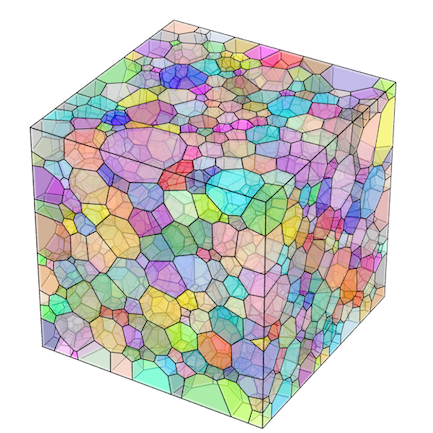
\includegraphics[height=0.4\textwidth]{pngFigures/cube460mm_100x100_croped.png}}
  \subcaptionbox{Onde plane incidente \label{subfig:ondePlane}}{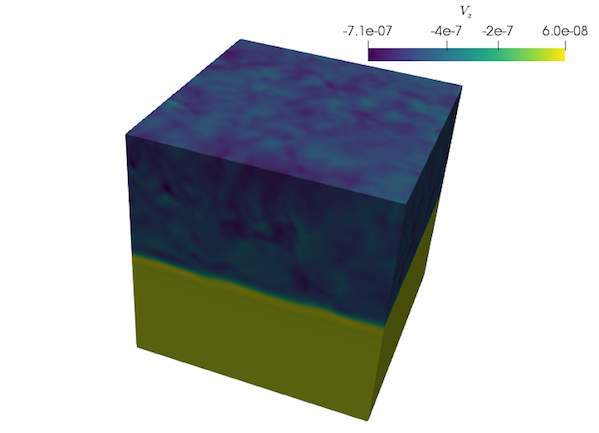
\includegraphics[height=0.4\textwidth]{pngFigures/velocity_100_croped.png}}
  % \caption{(\subref{subfig:microstructure}) Exemple de microstructure générée avec le logiciel \textsc{Neper} -- (\subref{subfig:ondePlane}) propagation d'une onde plane dans la microstructure \subref{subfig:microstructure}.}
  \caption{Exemple de microstructure générée avec le logiciel \textsc{Neper} et effet de l'anisotropie et de l'hétérogénéité des propriétés mécaniques sur la propagation d'une onde plane.}
  \label{fig:microStruct}
\end{figure}
%% chargement à spectre large
Les solutions en déplacement et vitesse calculées pour chaque milieu sur la face chargée ou sur la face opposée sont ensuite passées dans le domaine fréquentiel et comparées de sorte à tracer des courbes d'évolution du coefficient $\alpha$ en fonction de la fréquence.

Sur le plan théorique, on montre que le coefficient d'atténuation peut être exprimé pour les microstructures bimodales comme une somme de contributions provenant de chaque famille de grains.
Ces dernières étant pondérées par la fraction volumique correspondante.
Les résultats numériques obtenus sont en accord avec cette propriétés, comme en témoignent les courbes de la figure \ref{fig:attenuation}.
Ces courbes résultent de calculs théoriques et numériques dans une microstructure bidimensionnelle comportant deux tailles de grains caractérisées par les diamètres équivalents $\left\langle d \right\rangle =\{80,240\} \: \mu m$.
Les différences observables entre les figures \ref{fig:test} et \ref{fig:test_num} s'expliquent par le fait que la théorie est basée sur l'hypothèse de diffusion simple des ondes (\textit{i.e. une seule réflexion des ondes}), tandis que la modélisation numérique prend en compte la diffusion multiple. 
On voit qu'à mesure que la fraction volumique de gros grains $F_{GG}$ décroit (\textit{resp. augmente}), la courbe d'atténuation se rapproche du cas d'une microstructure monomodale constituée uniquement de petits (\textit{resp. gros}) grains.
%%
% Les premiers résultats numériques obtenus montrent que lorsque la distribution de diamètre équivalent dans la microstructure est bimodale, les courbes $\alpha(f)$ et $\beta(f)$ changent avec la fraction volumique de gros grains (FGG).
% La figure \ref{fig:attenuation} illustre ce dernier point pour l'atténuation sur un cas bidimensionnel dans lequel les deux tailles de grain considérées sont $\left\langle d \right\rangle =\{80,240\} \: \mu m$.
\begin{figure}[h!]
  \centering
  {\phantomsubcaption{\label{fig:test}}}
  {\phantomsubcaption{\label{fig:test_num}}}
  \begin{tikzpicture}% ,yticklabels at=edge left,ylabels at=edge left
  \begin{groupplot}[group style={group size=2 by 1,horizontal sep=3ex,vertical sep=1ex,yticklabels at=edge left,ylabels at=edge left,xticklabels at=edge bottom,xlabels at=edge bottom}
    % ,ymajorgrids=true,xmajorgrids=true,axis on top%,scale only axis,
    ,width=0.5\textwidth
    ,xlabel=$f$(MHz),ylabel=$\alpha$(1/m)
    ,ymin=0,xmin=0
    %,xmax=20
    ,ymax=140
    % ,ymax=220
    ]
    
    
    \nextgroupplot[title={(a) Théorique}]
    %% 240-80
    
    
    \addplot[black!50,thick] table[x expr=\thisrow{f}/1.e6,y=80mm] {pgfFigures/pgfFiles/bimodal_analytical2D.pgf};
    \addplot[black,thick] table[x expr=\thisrow{f}/1.e6,y=240mm] {pgfFigures/pgfFiles/bimodal_analytical2D.pgf};

    % \addplot[Blue,only marks,mark repeat=3,mark=+,thick] table[x expr=\thisrow{f}/1.e6,y=240_80mm_25] {pgfFigures/pgfFiles/bimodal_analytical2D.pgf};
    \addplot[Blue,thick,densely dotted] table[x expr=\thisrow{f}/1.e6,y expr=0.75*\thisrow{80mm}+0.25*\thisrow{240mm}] {pgfFigures/pgfFiles/bimodal_analytical2D.pgf};

    % \addplot[Green,only marks,mark repeat=3,mark=x,thick] table[x expr=\thisrow{f}/1.e6,y=240_80mm_50] {pgfFigures/pgfFiles/bimodal_analytical2D.pgf};
    \addplot[Green,thick] table[x expr=\thisrow{f}/1.e6,y expr=0.5*\thisrow{80mm}+0.5*\thisrow{240mm}] {pgfFigures/pgfFiles/bimodal_analytical2D.pgf};

    %\addplot[Red,only marks,mark repeat=3,mark=asterisk,thick] table[x expr=\thisrow{f}/1.e6,y=240_80mm_75] {pgfFigures/pgfFiles/bimodal_analytical2D.pgf};
    \addplot[Red,thick, dashed] table[x expr=\thisrow{f}/1.e6,y expr=0.25*\thisrow{80mm}+0.75*\thisrow{240mm}] {pgfFigures/pgfFiles/bimodal_analytical2D.pgf};

    % \node[right,Red] at (15,68) {\scriptsize $\epsilon=3\%$};
    % \node[right,Green] at (15,84.2) {\scriptsize $\epsilon=4\%$};
    % \node[right,Blue] at (15,103.52) {\scriptsize $\epsilon=2\%$};

    
    \nextgroupplot[title={(b) Numérique},legend style={at={($(.75,-0.3)+(0.5cm,0.35cm)$)},legend columns=5}]
    %% 160-80

    \addplot[black!50,thick] table[x expr=\thisrow{f}/1.e6,y=FLG0] {pgfFigures/pgfFiles/bimodal160_80_2D.pgf};
    \addplot[black,thick] table[x expr=\thisrow{f}/1.e6,y=FLG100] {pgfFigures/pgfFiles/bimodal240_160_2D.pgf};

    \addplot[Blue,thick,densely dotted] table[x expr=\thisrow{f}/1.e6,y=FLG25] {pgfFigures/pgfFiles/bimodal240_80_2D.pgf};
    
    \addplot[Green,thick] table[x expr=\thisrow{f}/1.e6,y=FLG50] {pgfFigures/pgfFiles/bimodal240_80_2D.pgf};
    
    \addplot[Red,thick,dashed] table[x expr=\thisrow{f}/1.e6,y=FLG75] {pgfFigures/pgfFiles/bimodal240_80_2D.pgf};
    


    \addlegendentry{ $F_{GG}=0$}
    \addlegendentry{ $F_{GG}=1$}

    \addlegendentry{ $F_{GG}=0.25$}
    % \addlegendentry{$\alpha_{Th}$ $F_{GG}=0.25$}
    % \addlegendentry{Expected $F_{GG}=0.25$}

    \addlegendentry{ $F_{GG}=0.50$}
    % \addlegendentry{$\alpha_{Th}$ $F_{GG}=0.50$}
    % \addlegendentry{Expected $F_{GG}=0.50$}

    \addlegendentry{ $F_{GG}=0.75$}
    %\addlegendentry{$\alpha_{Th}$ $F_{GG}=0.75$}
    %\addlegendentry{Expected $F_{GG}=0.75$}

    
  \end{groupplot}
\end{tikzpicture}



%%% Local Variables:
%%% mode: latex
%%% TeX-master: "../manuscript"
%%% End:

  \caption{{\'E}volution du coefficient d'atténuation en fonction de la fréquence pour des microstructures 2D unimodales et bimodales: comparaison entre les prédictions théoriques et les résultats numériques. L'influence de la Fraction volumique de Gros Grains ($F_{GG}$) est mise en évidence.}
  \label{fig:attenuation}
\end{figure}
% En particulier, les courbes semblent tendre vers celles des deux distributions unimodales pour les cas limites $FGG \rightarrow 0$ et $FGG \rightarrow 100 \%$.

%En appliquant la procédure à différentes microstructures (bi- ou tridimensionnelles, avec ou sans concentration de gros grains dans certaines régions, \textit{etc.}), l'idée est de déduire un maximum d'informations des courbes $\alpha(f)$ et $\beta(f)$ par comparaison avec le modèle unimodal.

{\`A} partir de ces résultats, une procédure de caractérisation des distributions bimodales de la taille de grain a été proposée.
Elle consiste, à partir d'une courbe d'atténuation obtenue sur une microstructure, à résoudre un problème d'optimisation à trois paramètres basé sur les prédictions théoriques monomodales.
Les trois paramètres étant la fraction volumique de gros grains, le diamètre équivalent moyen des gros grains et celui des petits grains, les microstructures bimodales peuvent être caractérisées.
Cette approche conduit à des résultats satisfaisants pour peu que les courbes monomodales utilisées comme référence dans le problème d'optimisation soient bien représentatives de la réalité.
On peut donc imaginer utiliser un grand nombre de courbes d'atténuation expérimentales pour un matériau donné afin d'\textit{alimenter} le problème d'optimisation et obtenir des caractérisation de plus en plus précises.
Ceci ne constitue toutefois pour l'instant qu'une perspective de ces travaux.

\paragraph{Publication associée:}
$\newline$ 
\begin{itemize}
\item A. Renaud, B. Tie, J.H Schmitt and A.S. Mouronval, ``Multi-parameter optimization of attenuation data for characterizing grain size distributions and application to bimodal microstructures'', Ultrasonics, \textit{Soumis le 21/11/20 -- révision mineure requise le 16/02/21}
\end{itemize}




%%% Local Variables:
%%% mode: latex
%%% TeX-master: "main"
%%% End:

  \printbibliography[heading=subbibliography]
\end{refsection}

\begin{refsection}
  \subsection{Simulations numériques de dynamique des dislocations par le modèle discret/continu}
  \label{sec:post-doc_CEA}
  Depuis mon intégration du CEA au LC2M en Octobre dans le cadre d'un nouveau postdoc, je m'intéresse à l'influence des défauts nanométriques dans les métaux sur le comportement plastique à l'échelle macroscopique.
Cette étude s'inscrit dans le cadre de la conception des futurs réacteurs à fission et fusion et vise à clarifier les effets de l'irradiation d'aciers sur l'écrouissage, la localisation, la fragilisation, \textit{etc.}
Dans ce contexte, la Dynamique des Dislocations (DD) \cite{Zbib2012_DDD} est un outil numérique qui permet d'étudier l'interaction des dislocations avec les défauts d'irradiation à l'échelle microscopique et de comprendre l'influence sur le comportement à l'échelle du grain.
Néanmoins, la DD requiert, en accord avec la théorie des dislocations, le calcul des actions réciproques entre tous les segments des dislocations discrétisées présentes dans le domaine d'étude.
Il s'en suit que cette méthode est très coûteuse en terme de temps de calcul pour des volumes élémentaires représentatifs contenant un grand nombre de défauts.


\paragraph{Motivations/Objectifs:}
$\newline$
Le Modèle Discret/Continu (DCM) \cite{lemarchand2001_DCM,jamond2016_DCM} permet de contourner les difficutlés liées au coût de calcul caractéristiques des simulations DD.
Dans cette approche, le mouvement des dislocations et les aires que ces dernières balaient sont traduites en terme de déformations plastiques qui sont distribués sur les points de Gauss d'un maillage éléments finis.
Cet étalement de la déformation plastique permet de régulariser la discontinuité du déplacement résultant du mouvement des dislocations.
La résolution éléments finis apparaît alors comme une étape de relaxation visant à équilibrer les déformations plastiques en tenant compte des conditions aux limites.
Toutefois, l'étape de régularisation conduit à une mauvaise estimation du champ de contrainte dans le voisinage des dislocations (pour des distances de l'ordre de la taille du maillage), de sorte qu'une correction provenant de la DD est utilisée localement.
Les contraintes ainsi déterminées donnent accès aux forces de Peach-Köhler dont on déduit l'évolution du réseau de dislocations.

Récemment, une formulation de la DCM dans laquelle une approche de type Transformées de Fourier Rapides (FFT) remplace la méthode des éléments finis a été proposée \cite{bertin2015_fft}.
\begin{figure}[h!]
  \centering
  \subcaptionbox{Configuration initiale \label{subfig:disloc_ini}}{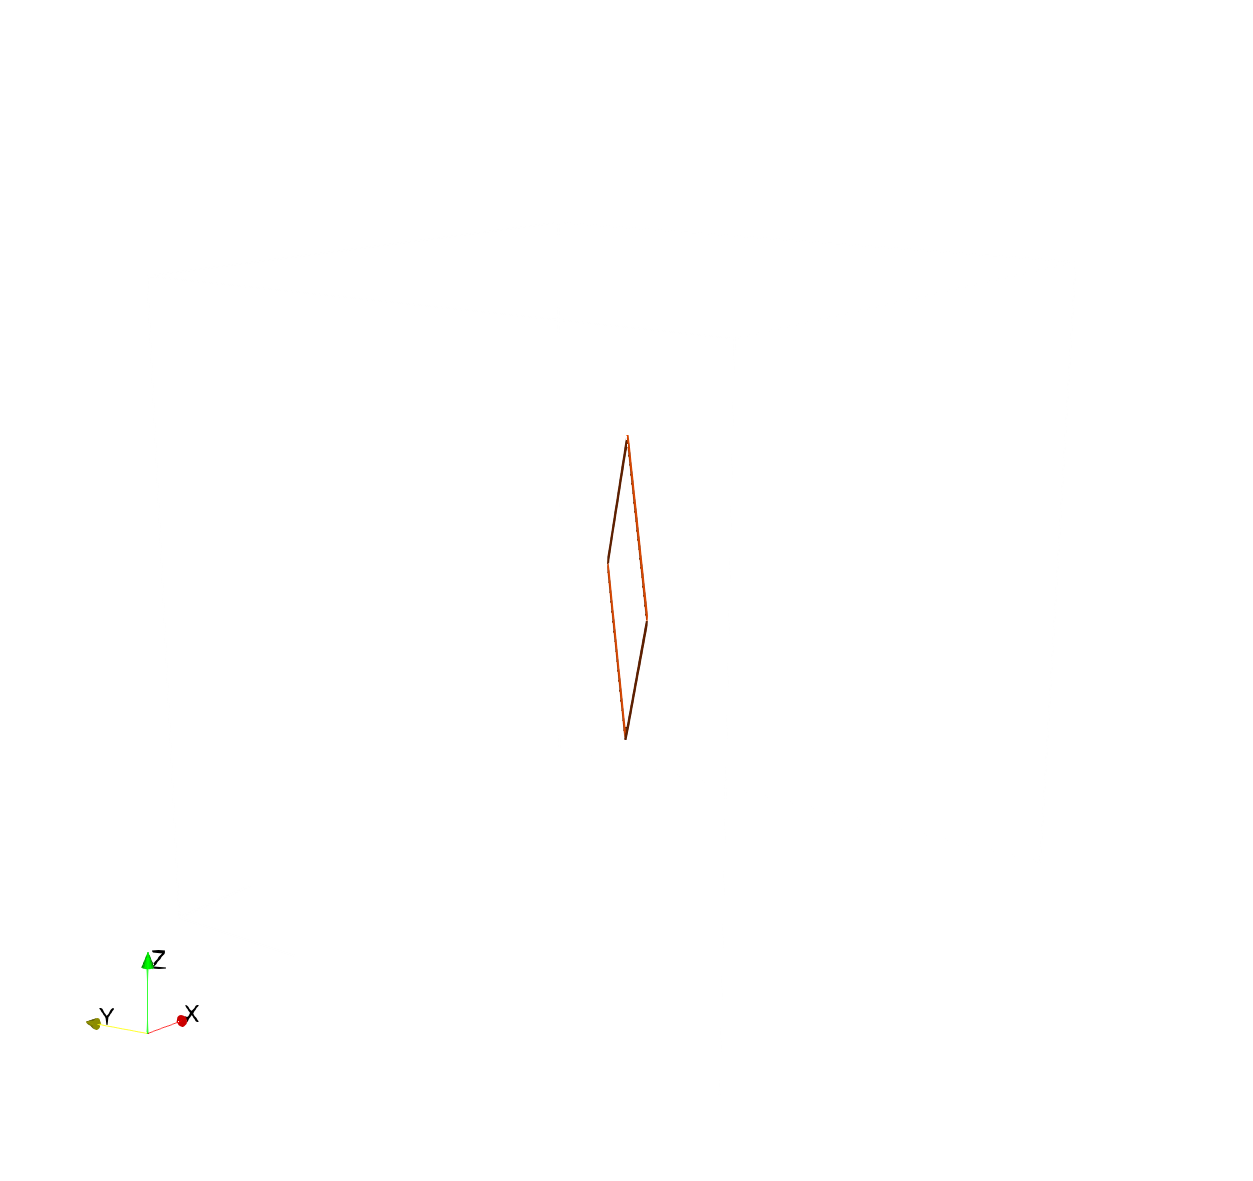
\includegraphics[trim=0 0 0 4cm, clip,height=0.4\textwidth]{pngFigures/initial_disloc.png}}
  \subcaptionbox{Configuration finale \label{subfig:disloc_fini}}{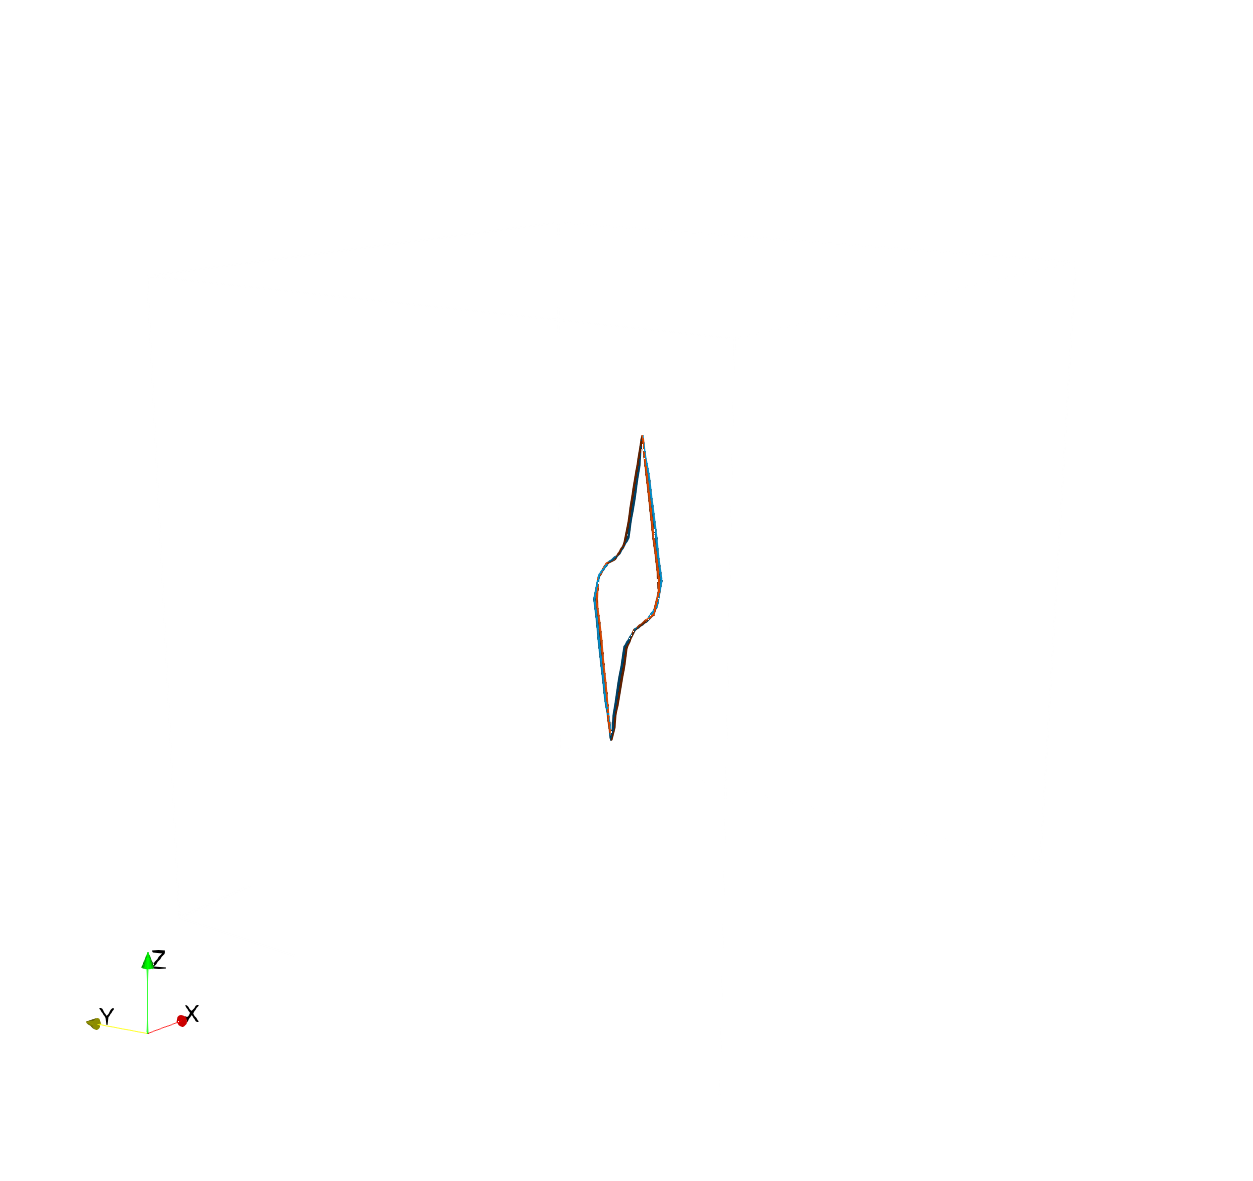
\includegraphics[trim=0 0 0 4cm, clip,height=0.4\textwidth]{pngFigures/final_disloc.png}}
  %\subcaptionbox{Configuration initiale (zoom)\label{subfig:disloc_ini}}{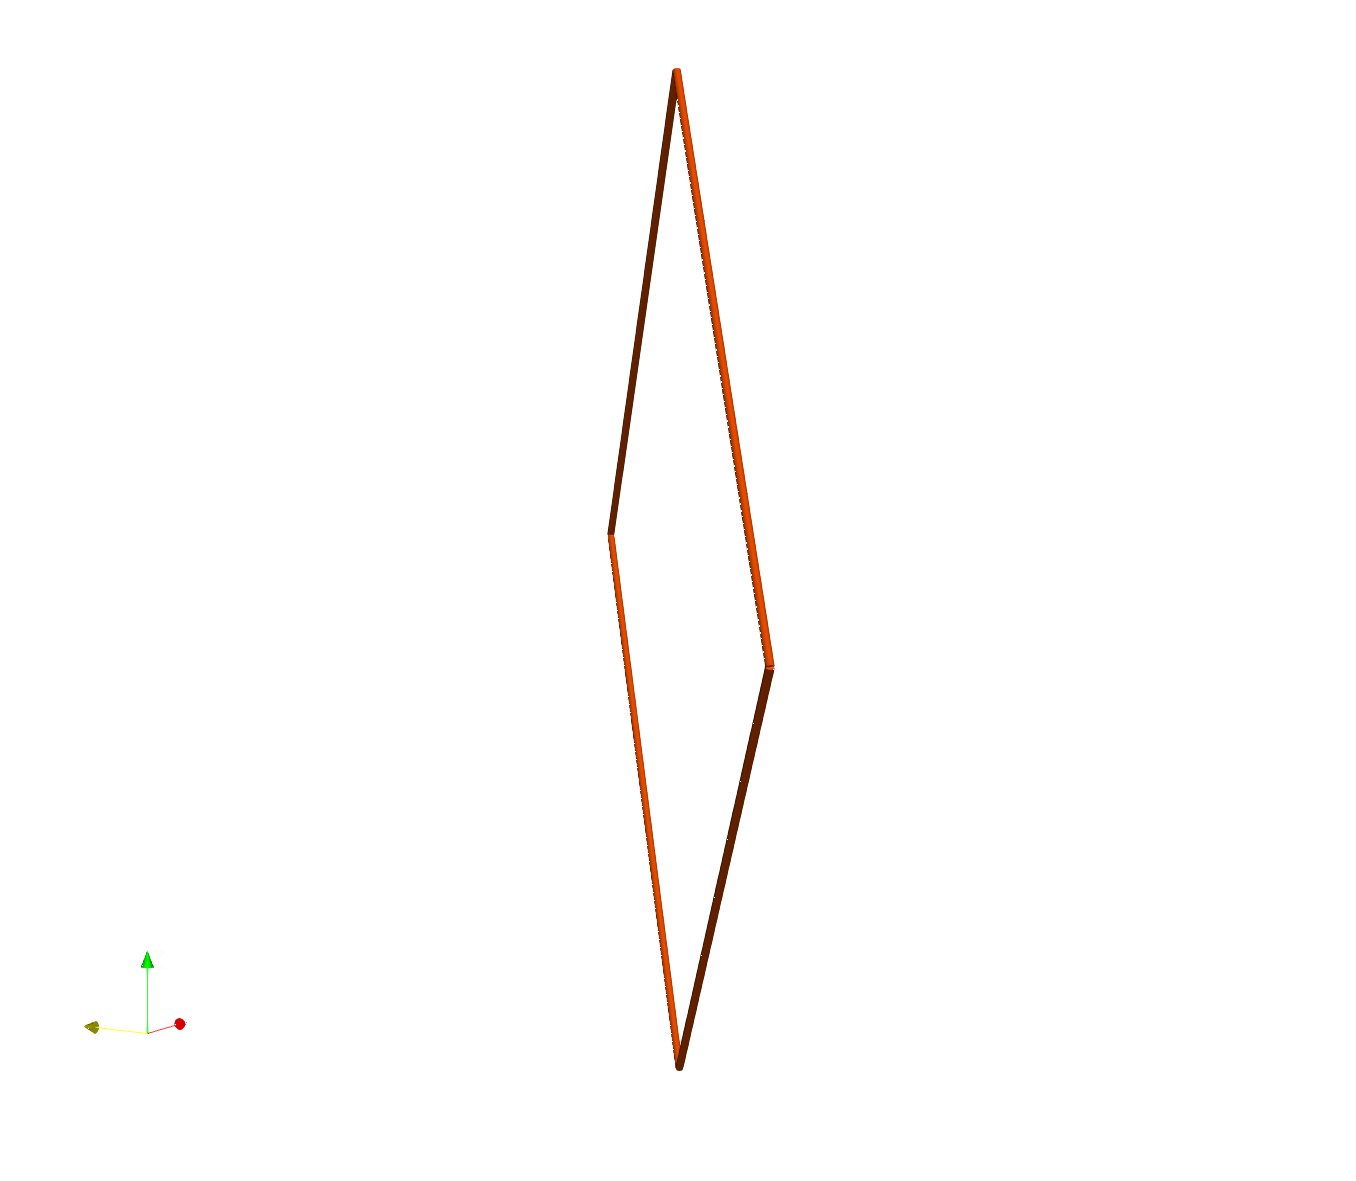
\includegraphics[height=0.4\textwidth]{pngFigures/initial_disloc_zoom.png}}
  %\subcaptionbox{Comparaison des contraintes sur la configuration finale \label{subfig:disloc_fini_stress}}{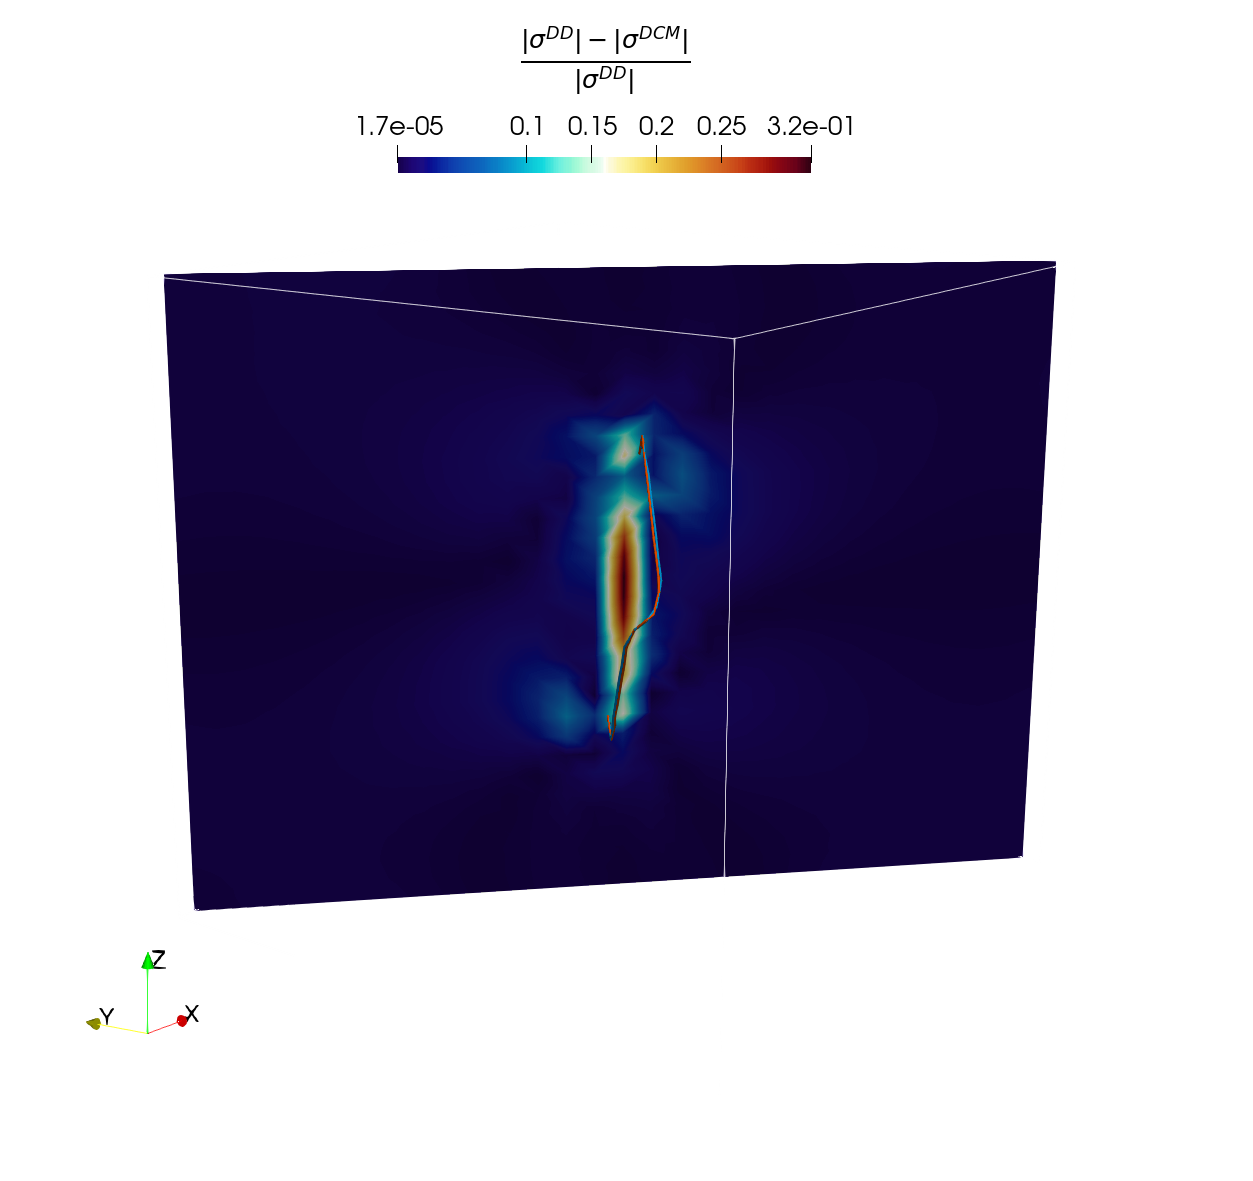
\includegraphics[height=0.6\textwidth]{pngFigures/final_disloc_stress.png}}
  % \caption{(\subref{subfig:microstructure}) Exemple de microstructure générée avec le logiciel \textsc{Neper} -- (\subref{subfig:ondePlane}) propagation d'une onde plane dans la microstructure \subref{subfig:microstructure}.}
  \caption{{\'E}volution d'une boucle prismatique $\vect{b}=3(\vect{e}_y - \vect{e}_x)$ dans un domaine soumis à une contrainte de cisaillement homogène $\sigma_{yz} = \sigma_d$. Comparaison entre la solution DD pure (ligne orange) et la solution DCM (ligne bleue).}
  \label{fig:comparisonDCM}
\end{figure}
Le couplage DD-FFT vise essentiellement à résoudre des problèmes sur des grilles très fines en profitant de la grande rapidité de calcul offerte par l'algorithme FFT.
Dans ces travaux, cette formulation de la DCM sera considérée en couplant les codes \textit{Amitex} \cite{Amitex_FFT} et \textit{Numodis} \cite{Numodis}, tous deux développés au CEA pour les parties FFT et DD respectivement.
Le premier objectif de mon postdoc a été de terminer le couplage des deux codes afin d'obtenir des premières comparaisons satisfaisantes avec la DD seule.

La figure \ref{fig:comparisonDCM} montre un exemple de résultats obtenus sur un problème simple à titre d'illustration.
On considère une boucle de dislocation prismatique dans un cristal cubique à faces centrées supposé infini et soumis à une contrainte de cisaillement homogène $\sigma_{yz}$.
Sous l'action de cette contrainte, la dislocation se déforme et on compare les solutions calculées par la DCM et la DD pour s'assurer de la cohérence du couplage DD--FFT mis en place.

Les différences qui apparaissent dans l'évolution de la boucle prismatique évaluée par la DCM ou la DD, bien que faibles, s'explique premièrement par le choix de la procédure de régularisation des déformations plastiques qui n'est pas unique \cite{jamond2016_DCM,VATTRE2014,Capolungo2021}.
Par ailleurs, la DCM implique plusieurs paramètres algorithmiques jouant sur l'étalement des déformations plastiques et sur la taille de la zone où la correction DD est calculée.
Tout l'intérêt de ces paramètres est de pouvoir assurer un équilibre entre précision et efficacité de l'approche DCM.
Toutefois, aucune analyse numérique n'a permis à ce jour de déterminer de valeurs optimales pour ces derniers.

Le premier objectif de mon travail est donc l'analyse numérique du schéma DCM afin d'extraire des valeurs optimales de ces coefficients, en analysant les équations dans un premier temps, et en recourant à des simulations dans un second temps.
% On considère ici une boucle de dislocation prismatique contenue dans le plan de normale $\vect{n} = \vect{e}_y - \vect{e}_x$ dans un cristal cubique à faces centrées dont les axes cristallographiques sont alignés avec le repère global.
% Le vecteur de Burgers de cette dislocation est $\vect{b}=3\vect{n}$, de sorte que la boucle ne peut se mouvoir que dans la direction $\vect{n}$.
% Le domaine est soumis à une contrainte de cisaillement $\sigma_{yz}$ et le déplacement de la dislocation sous l'effet de ce chargement est calculée par la DCM d'une part et la DD d'autre part pour comparaison.


% Bien que la DCM permet de calculer des solutions proches de celles de la DD, le choix de la procédure de régularisation des déformations plastiques utilisée n'est pas unique \cite{jamond2016_DCM,VATTRE2014,Capolungo2021}, ce qui peut conduire à une précision variable de la méthode.
% Par ailleurs, la définition de la zone dans laquelle la correction DD est calculée repose sur un certain nombre de paramètres algorithmiques inteviennent, ces derniers permettent de régler la taille du domaine dans lequel la correction DD est calculée.

% \cite{bertin2015_fft,Capolungo2021,VATTRE2014}

% \begin{itemize}
% \item Défauts d'irradiation à l'échelle atomique
% \item Influence de ces défauts sur la plasticité (à travers leur interaction avec les dislocations) et modification du comportement plastique à l'échelle mésoscopique
% \item Le lien entre ces interactions et les comportements macroscopiques (écrouissage, localisation, fragilisation) n'est toutefois pas encore complètement clair. De sorte que ce sujet fait l'objet de beaucoup de recherches mutli-échelle
% \item Une méthode numérique permettant de simuler ce genre de problème est la méthode des dislocations discrète ... (description)
% \item Cette dernière est néanmoins limitées pour des raisons de coûts de calcul, à des problèmes impliquant des petites dimensions du domaines d'étude.
% \item Récemment, une approche couplant la DDD avec des méthodes adaptées à l'échelle macroscopique (FEM, FFT, \textit{etc.}) a été proposée. Parler des aires balayées par les dislocations dont on déduit les déformations plastiques, qui sont étalées dans le maillage afin de régulariser la discontinuité du déplacement résultant du mouvement des dislocation. La résolution éléments finis apparaît alors comme une étape de relaxation visant à relaxer les déformations plastiques en tenant compte des conditions aux limites.
  % {\`A} cause de la régularisation, le champ de contrainte calculé par la méthode macroscopique peine à capturer la solution analytique dans le voisinage des dislocations (pour des distances de l'ordre de la taille du maillage).
  % On utilise alors la contrainte calculée par la DDD pour corriger la solution proche des dislocations.
% \end{itemize}


\paragraph{Objectifs:}
% $\newline$
% \begin{itemize}
% \item Terminer et valider le couplage
% \item Optimisation des paramètres de la méthode $\rightarrow$ analyse numérique (illustrer ça par des figures)
% \item Exploitation du modèle sur des simulations à grande échelle pour l'étude de l'effet des défauts d'irradiation sur l'écoulement plastique (modèle de comportement homogénéisé)
% \end{itemize}


\begin{itemize}
\item expliquer le contexte / la problématique
\item la méthode DCM et ses grands principes
\item mon travail là-dedans et les objectifs fixés/remplis à ce jour.
\end{itemize}
%%% Local Variables:
%%% mode: latex
%%% TeX-master: "main"
%%% End:

  \printbibliography[heading=subbibliography]
\end{refsection}

\subsection{Résumé court}
\label{resume_recherche}

%% Rappel
% stage
% Mes premiers travaux de recherche portaient sur la simulation numérique du procédé de soudage par friction/malaxage afin de mettre en évidence l'extrusion de couches de matière due à un défaut d'excentrement de l'outil.
% Le modèle proposé prenait en compte les couplages thermo-mécaniques dans un cadre Eulérien.
% L'interface outil/matière et la cinématique de l'outil comprenant un mouvement d'excentrique étaient modélisées par des fonctions de niveau combinées à la méthode X-FEM.

$\newline$
% doctorat
Mes activités de doctorat concernaient les procédés de mise en forme de matériaux métalliques à haute vitesse, et plus précisément l'évaluation des états résiduels.

Sur le plan numérique, j'ai étendu la Méthode des Points Matériels à l'approximation de Galerkin Discontinue afin de développer une méthode numérique originale, la DGMPM.
La combinaison d'une discrétisation spatiale adaptée aux grandes transformations et de solveurs de Riemann pour le calcul des flux permet de suivre précisément les ondes dans les solides se déformant beaucoup.

Par ailleurs, bien que les ondes plastiques gouvernent les états résiduels, leur influence n'est en général pas bien comprise.
J'ai donc étudié la structure caractéristique des systèmes hyperboliques pour des cas de déformations et de contraintes planes dans des solides élasto-plastiques en petites déformations.
La contribution majeure de cette analyse est la construction des trajets de chargement suivis à travers les ondes plastiques.


$\newline$
% postdoc
Je m'intéresse en ce moment, dans le cadre de mon postdoc, au contrôle non-destructif par ultrasons des matériaux polycristallins.
%
L'objectif est de proposer une approche expérimentale de caractérisation les distributions bimodales de taille de grain.
L'approche consiste à combiner les modèles théoriques d'atténuation et de diffusion des ondes élastiques, bien adaptés aux distributions unimodales, avec les résultats de simulations numériques, nécessitant par ailleurs le recours au calcul hautes performances.




$\newline$
%% Pourquoi ca fit le profil
% développement  de  modèles  prédictifs  
Mes activités de recherche ont toutes pour objectif le développement de modèles prédictifs théoriques, numériques ou expérimentaux, s'appuyant sur la physique, les mathématiques appliquées et la science des matériaux.
% Cette  problématique (instabilité) inclut  les  travaux  portant  sur  l'intégrité  des  matériaux  et  des  structures  en  lien  avec  les  hétérogénéités constitutives aux différentes échelles.
Ces travaux prennent en compte les hétérogénéités à différentes échelles dans le cadre de la dynamique des solides, ce qui me paraît complémentaire avec les activités du laboratoire.

Aussi, je pense que mon profil est en parfaite adéquation avec le poste de Maître de conférences proposé à l'institut Jean le Rond d'Alembert.

\paragraph{Mots-clés:}Plasticité, Matériaux hétérogènes,  Dynamique  des  structures, Modélisation numérique, Analyse numérique.

%%% Local Variables:
%%% mode: latex
%%% TeX-master: "main"
%%% End:
